% ===== block5-computing-clusters.tex: "Computing clusters", weekend 2, the Friday 16:00 block "Large-scale computing" =====
% (the Saturday 08:15 block until 2026-11-11, when Carlos merged it with parallelized matrix factorization)
% A port into Codex plates of the first block of FDD weekend 7, "The cost of computation and supercomputers"
% (git_fdd/projects/weekend-07-large-scale/carlos-lectures/slides/w7-cost-slides.tex, commit b296f78),
% with the cuts and changes Carlos dictated on 2026-11-10. README.md has the frame by frame map.
% Every number is FDD's (its NUMBERS.md, sections A and G), except the platform facts of
% alps-platform-frame.tex, each listed with its source in tools/check_port.py, which checks both.
% "FDD slide N" below is the number printed on FDD's slide (title 1, section dividers counted).
% Build and check from this folder:
%   ../style/tools/build.sh block5-computing-clusters.tex
%   ../style/tools/check.sh block5-computing-clusters.pdf
%   python3 ../style/tools/check_overlays.py block5-computing-clusters.pdf
%   python3 tools/check_port.py
\documentclass[aspectratio=169]{beamer}
% Copied on 2026-11-03 from eth-ainit-hs26/w1-lecture-material, commit 9792819, file style/ainit-preamble.tex. To pull a fix, diff against the source and recopy.
% ===== ainit-preamble.tex: the official deck style of AI in Industry (AINIT), HS26 =====
% "Codex plates". Chosen by Carlos on 9 October 2026 from a two round style board. Round one
% had Codex, Atlas, Spec sheet, Sheet and Cartridge; round two had Codex violet, Codex plates,
% Vellum atlas and Cool atlas. CLAUDE.md in this folder records the decision, the rules and the
% traps. Read it before changing anything here.
%
% What it is. Every slide is a leaf of a codex: warm vellum inside a fine double ruled block,
% pricking dots in the outer margin, the title above a double rule, a violet folio and an italic
% slug in the lower margin. The figures speak a technical grammar in fine ink: sharp rectangles,
% 45 degree hatching in violet lines with no solid fill, dashed outlines for whatever is refused
% or not taken, right angled connectors, numbered balloons on hairline leaders, and a large
% numeral in a heavy square. Violet is the rubric: the folio, key words, the chosen path, the
% current weekend. Ochre is the second accent. Ge'ez numerals number the games, the balloons and
% the sections, from one to five. Arabic digits take over beyond five, because five is how many
% numerals the room learns in the Ge'ez games.
%
% Each deck does:
%   \documentclass[aspectratio=169]{beamer}
%   % Copied on 2026-11-03 from eth-ainit-hs26/w1-lecture-material, commit 9792819, file style/ainit-preamble.tex. To pull a fix, diff against the source and recopy.
% ===== ainit-preamble.tex: the official deck style of AI in Industry (AINIT), HS26 =====
% "Codex plates". Chosen by Carlos on 9 October 2026 from a two round style board. Round one
% had Codex, Atlas, Spec sheet, Sheet and Cartridge; round two had Codex violet, Codex plates,
% Vellum atlas and Cool atlas. CLAUDE.md in this folder records the decision, the rules and the
% traps. Read it before changing anything here.
%
% What it is. Every slide is a leaf of a codex: warm vellum inside a fine double ruled block,
% pricking dots in the outer margin, the title above a double rule, a violet folio and an italic
% slug in the lower margin. The figures speak a technical grammar in fine ink: sharp rectangles,
% 45 degree hatching in violet lines with no solid fill, dashed outlines for whatever is refused
% or not taken, right angled connectors, numbered balloons on hairline leaders, and a large
% numeral in a heavy square. Violet is the rubric: the folio, key words, the chosen path, the
% current weekend. Ochre is the second accent. Ge'ez numerals number the games, the balloons and
% the sections, from one to five. Arabic digits take over beyond five, because five is how many
% numerals the room learns in the Ge'ez games.
%
% Each deck does:
%   \documentclass[aspectratio=169]{beamer}
%   % Copied on 2026-11-03 from eth-ainit-hs26/w1-lecture-material, commit 9792819, file style/ainit-preamble.tex. To pull a fix, diff against the source and recopy.
% ===== ainit-preamble.tex: the official deck style of AI in Industry (AINIT), HS26 =====
% "Codex plates". Chosen by Carlos on 9 October 2026 from a two round style board. Round one
% had Codex, Atlas, Spec sheet, Sheet and Cartridge; round two had Codex violet, Codex plates,
% Vellum atlas and Cool atlas. CLAUDE.md in this folder records the decision, the rules and the
% traps. Read it before changing anything here.
%
% What it is. Every slide is a leaf of a codex: warm vellum inside a fine double ruled block,
% pricking dots in the outer margin, the title above a double rule, a violet folio and an italic
% slug in the lower margin. The figures speak a technical grammar in fine ink: sharp rectangles,
% 45 degree hatching in violet lines with no solid fill, dashed outlines for whatever is refused
% or not taken, right angled connectors, numbered balloons on hairline leaders, and a large
% numeral in a heavy square. Violet is the rubric: the folio, key words, the chosen path, the
% current weekend. Ochre is the second accent. Ge'ez numerals number the games, the balloons and
% the sections, from one to five. Arabic digits take over beyond five, because five is how many
% numerals the room learns in the Ge'ez games.
%
% Each deck does:
%   \documentclass[aspectratio=169]{beamer}
%   \input{../style/ainit-preamble}      % this file
%   \input{../style/ainit-course}        % the facts of the course and the three weekends frame
%   \renewcommand{\deckslug}{AI in Industry, weekend 1}
% and is compiled with lualatex FROM the deck's own directory, three times: the leaf, the dots
% and the balloons are placed with remember picture and settle on the third pass. Fonts are
% EB Garamond, Garamond Math and Libertinus Mono (all in TeX Live) and Kefa III for Ethiopic
% (a macOS system font; set \geezfontpath before this file to use another folder).
%
% What a deck sets:
%   \title \subtitle \author \institute \date       the title page
%   \renewcommand{\deckslug}{...}                   the italic slug in the footer
%   \def\titlegeez{...}                             optional: a Ge'ez line above the cover title
%   \plateImage \plateCredit \quoteText \quoteCitation   the cold open, shown by \coldopenframe
% Frames 'title' and 'cold open' are [plain,noframenumbering]; a \section makes its own divider.
%
% The kit a deck may use:
%   macros   \hl{key words}  \geez{...}  \geezNumeral{n}  \cxballoon  \treelink  \weblink  \qrlink
%            \framedimgh{height}{file}  \coldopenframe  \begin{codeplate}...\end{codeplate}
%            \begin{cxlist}[\small]...\end{cxlist}  a denser list for reference slides
%   styles   chip, chip strong, chip dim, edge strong, edge dim, elab, elab dim, axis, vec a,
%            vec b, vlab a, vlab b, anglearc, anglelab, gloss, hatch, hatch fine
%   colours  paper ink muted brand accent2 good bad ruling ruledark nib
%
% House rules that bind every deck (the lecture-slides skill has the long form):
%   light and projection first; no red against green (good is blue, bad is vermillion); no ALL
%   CAPS; no dash or double hyphen in prose; nothing under a diagram; a section divider carries a
%   numeral, "Section N", the title and a band, nothing else; only the title page names the
%   lecturer; the only number in the chrome is the folio; no cell grids, column letters, tabs,
%   title blocks or arcade chrome. Never name a colour fg or bg: beamer rebinds both.

\usepackage{fontspec}
\usepackage{amsmath}
\usepackage{booktabs}
\usepackage{unicode-math}
\usefonttheme{professionalfonts}
\usefonttheme{serif}
\usepackage{tikz}
\usetikzlibrary{arrows.meta, positioning, calc, backgrounds, fit, overlay-beamer-styles,
                decorations.pathreplacing, patterns.meta}
\setbeamertemplate{navigation symbols}{}

% === type: EB Garamond (TeX Live), Garamond-Math for the maths, Kefa III for Ethiopic ===
\setmainfont{EBGaramond}[
  Extension      = .otf,
  UprightFont    = *-Medium,
  ItalicFont     = *-MediumItalic,
  BoldFont       = *-SemiBold,
  BoldItalicFont = *-SemiBoldItalic,
  Ligatures      = TeX,
  Numbers        = Lining,
  Scale          = 1.08]
\setmathfont{Garamond-Math.otf}[Scale=1.08]
% a monospaced face for code and addresses, sized to the lowercase of the main face
\setmonofont{LibertinusMono-Regular.otf}[Scale=MatchLowercase]

% Kefa III is a macOS system font. Its light and bold instances are variable font instances.
% Without the file, the deck still compiles: Ge'ez text then lacks glyphs and a warning says so.
\providecommand{\geezfontpath}{/System/Library/Fonts/Supplemental/}
\IfFileExists{\geezfontpath KefaIII.ttf}{%
  \newfontfamily\geezfont[Path=\geezfontpath]{KefaIII.ttf}
  % the light instance, for large numerals
  \newfontfamily\geezlightfont[Path=\geezfontpath, RawFeature={instance=Light}]{KefaIII.ttf}
  % the bold instance, for the numerals in balloons (the regular weight is too thin there)
  \newfontfamily\geezboldfont[Path=\geezfontpath, RawFeature={instance=Bold}]{KefaIII.ttf}
}{%
  \PackageWarningNoLine{ainit-preamble}{Kefa III was not found in \geezfontpath. Ge'ez text
    will lack glyphs. Set \string\geezfontpath\space before this file.}%
  \newcommand{\geezfont}{}\newcommand{\geezlightfont}{}\newcommand{\geezboldfont}{}}
\newcommand{\geez}[1]{{\geezfont #1}}
\newcommand{\geezlight}[1]{{\geezlightfont #1}}

% === colours. Never name one fg or bg (beamer rebinds both). ===
\definecolor{paper}{HTML}{F9F4E3}     % vellum, lightness above 93 percent
\definecolor{ink}{HTML}{241F1A}       % warm black, iron gall
\definecolor{muted}{HTML}{5E5448}     % secondary text, darker than black!55
\definecolor{brand}{HTML}{58409A}     % violet in the rubric role
\definecolor{accent2}{HTML}{8F5A06}   % ochre, the second accent
\definecolor{good}{HTML}{0072B2}      % Okabe-Ito blue: a win
\definecolor{bad}{HTML}{D55E00}       % Okabe-Ito vermillion: a loss. No red against green, ever.
\colorlet{ruling}{ink!40!paper}       % the ruled lines of the leaf
\colorlet{ruledark}{ink!62!paper}     % the heavier ruled lines
\colorlet{nib}{ink!88!paper}          % the outline ink of the figures

\setbeamercolor{normal text}{fg=ink, bg=paper}
\setbeamercolor{structure}{fg=brand}
\setbeamercolor{alerted text}{fg=brand}
\setbeamersize{text margin left=15mm, text margin right=15mm}

% === links: violet, and a raw address keeps the mono face, so a link is marked twice ===
% Beamer loads hyperref. The border is cleared; colorlinks stays off because it would also tint
% the section title on the divider.
\hypersetup{pdfborder={0 0 0}, breaklinks=true}
\urlstyle{tt}
\renewcommand{\UrlFont}{\ttfamily\color{brand}}
% \weblink{https://...}{the words the room reads}: an inline link whose visible text is prose.
\newcommand{\weblink}[2]{\href{#1}{\color{brand}#2}}

% \qrlink{2.6cm}{https://...}: a vector QR on a plain white plate in a hairline mount. The code is
% generated from the address at compile time, so it cannot disagree with the address printed
% beside it. Always print the address next to it.
% Two guards, both invisible in the source. nolink: qrcode makes the whole code a link by default,
% and a link is painted in the link colour. \color{black}: qrcode draws in the current colour, so
% on a full bleed frame where \color{white} is active the modules would vanish.
\usepackage{qrcode}
\newcommand{\qrlink}[2]{%
  \tikz{\node[inner sep=4pt, fill=white, draw=ruledark, line width=0.6pt, line join=miter]
    {\color{black}\qrcode[nolink, height=#1]{#2}};}}

% \framedimgh{2.5cm}{img/photo.jpg}: a photograph or figure of the given height in a hairline mount,
% standing 1.4 mm off the picture as the plate of the cold open does.
\newcommand{\framedimgh}[2]{%
  \tikz{\node[inner sep=1.4mm, draw=ruling, line width=0.4pt, line join=miter]
    {\includegraphics[height=#1]{#2}};}}

% === the overlay style used by every piece of page furniture ===
\tikzset{cx page/.style={remember picture, overlay, shift={(current page.north west)},
  x=1mm, y=-1mm}}

% === hatching: the one fill of the figures. Violet lines at 45 degrees, no solid colour under them ===
\tikzset{
  hatch/.style={pattern={Lines[angle=45, distance=0.95mm, line width=0.42pt]}, pattern color=brand},
  hatch fine/.style={pattern={Lines[angle=45, distance=0.62mm, line width=0.36pt]}, pattern color=brand},
}

% === Ge'ez numerals up to five, digits beyond ===
% The room learns ፩ to ፭ in the Ge'ez games (the course numbers the games with them).
\newcommand{\geezNumeral}[1]{\ifcase#1 0\or ፩\or ፪\or ፫\or ፬\or ፭\else\number#1\fi}
\newcommand{\cxnum}[1]{\ifnum#1<6\relax{\geezboldfont\geezNumeral{#1}}\else\number#1\fi}
\newcounter{glossn}

% a box that is scaled down to fit when its natural width exceeds #1, and left alone otherwise
\newsavebox{\cxfitbox}
\newcommand{\cxfit}[2]{%
  \sbox{\cxfitbox}{#2}%
  \ifdim\wd\cxfitbox>#1\relax\resizebox{#1}{!}{\usebox{\cxfitbox}}\else\usebox{\cxfitbox}\fi}

% === the footer slug: each deck renews it ===
\providecommand{\deckslug}{AI in Industry}

% === the leaf: ruled block with a fine double rule, pricking marks in the outer margin ===
\setbeamertemplate{background}{%
  \setcounter{glossn}{0}%
  \begin{tikzpicture}[cx page]
    \draw[ruling, line width=0.55pt] (8,5) rectangle (152,82);
    \draw[ruling, line width=0.25pt] (8.9,5.9) rectangle (151.1,81.1);
    \foreach \i in {0,...,12} {\fill[ruling] (3.2,{5+6.4167*\i}) circle (0.3);}
  \end{tikzpicture}}

% === the title sits above the first ruled line of the block; an over long title is scaled to fit ===
\setbeamertemplate{frametitle}{%
  \vbox to 17.5mm{\offinterlineskip
    \vskip 8.3mm
    \hbox to\textwidth{\vrule height 5.3mm depth 1.9mm width 0pt
      \cxfit{\textwidth}{\color{ink}\fontsize{19}{22}\selectfont\bfseries\insertframetitle}\hfil}%
    \vskip 0.8mm
    \hbox to\textwidth{\color{ruledark}\vrule height 0.7pt depth 0pt width\textwidth}%
    \vskip 0.6mm
    \hbox to\textwidth{\color{ruling}\vrule height 0.3pt depth 0pt width\textwidth}%
    \vss}}

% === the folio in the lower margin, the italic slug beside it ===
\setbeamertemplate{footline}{%
  \vbox to 8.2mm{\offinterlineskip\vss
    \hbox to\paperwidth{\hskip 15mm
      {\color{brand}\fontsize{12}{14}\selectfont\insertframenumber}\hskip 3.4mm
      {\color{muted}\footnotesize\itshape\deckslug}\hfil}%
    \vskip 2.2mm}}

% === the title page ===
% \titlegeez (a Ge'ez line over the title) and \geezYear (the year, in Ge'ez numerals, after the
% date) are optional. \geezYear comes from ainit-course.tex.
\setbeamertemplate{title page}{%
  \begin{tikzpicture}[cx page]
    \node[text=brand, font=\fontsize{17}{20}\selectfont, anchor=base] at (80,20.5)
      {\ifdefined\titlegeez\geez{\titlegeez}\fi};
    \node[text=ink, font=\fontsize{27}{30}\selectfont\bfseries, text width=104mm, align=center,
      anchor=north, inner sep=0] at (80,25) {\inserttitle};
    \draw[ruledark, line width=0.8pt] (62,50.5) -- (98,50.5);
    \draw[ruling, line width=0.3pt] (62,51.5) -- (98,51.5);
    \node[text=muted, font=\large\itshape, anchor=north, inner sep=0] at (80,55)
      {\insertsubtitle};
    \node[text=ink, font=\large, anchor=base, inner sep=0] at (80,67) {\insertauthor};
    \node[text=muted, font=\normalsize\itshape, anchor=base, inner sep=0] at (80,72.2)
      {\insertinstitute};
    \node[text=muted, font=\normalsize\itshape, anchor=base, inner sep=0] at (80,77.2)
      {\insertdate\ifdefined\geezYear\hspace{3.2mm}{\upshape\color{brand}\geez{\geezYear}}\fi};
  \end{tikzpicture}}

% === the section page: a numeral in a heavy square, Section N, the title, a hatched band ===
% The numeral is Ge'ez up to five and a digit beyond. A title that is wider than 92 mm at the
% display size wraps over several lines at a smaller size, and the band moves down under it.
\newif\ifcxwrap
\setbeamertemplate{section page}{%
  \sbox{\cxfitbox}{\fontsize{36}{40}\selectfont\bfseries\insertsectionhead}%
  \ifdim\wd\cxfitbox>92mm\relax\cxwraptrue\else\cxwrapfalse\fi
  \begin{tikzpicture}[cx page]
    \draw[brand, line width=1.8pt, line join=miter] (17,30.2) rectangle (44,57.2);
    \draw[brand, line width=0.4pt] (18.9,32.1) rectangle (42.1,55.3);
    \ifnum\insertsectionnumber<6\relax
      \node[text=brand, font=\fontsize{54}{54}\selectfont, anchor=center] at (30.56,43.7)
        {\geezlight{\geezNumeral{\insertsectionnumber}}};
    \else
      \node[text=brand, font=\fontsize{54}{54}\selectfont, anchor=center] at (30.56,43.7)
        {\number\insertsectionnumber};
    \fi
    \node[text=muted, font=\fontsize{14}{16}\selectfont\itshape, anchor=base west, inner sep=0]
      at (53,33.2) {Section \insertsectionnumber};
    \ifcxwrap
      \node[text=ink, font=\fontsize{26}{29}\selectfont\bfseries, anchor=north west, inner sep=0,
        text width=92mm, align=flush left] (cxst) at (53,36.5) {\insertsectionhead};
      \fill[hatch] ([shift={(0,3.4)}]cxst.south west) rectangle ([shift={(92,7)}]cxst.south west);
      \draw[brand, line width=0.5pt] ([shift={(0,3.4)}]cxst.south west) -- ++(92,0)
        ([shift={(0,7)}]cxst.south west) -- ++(92,0);
    \else
      \node[text=ink, font=\fontsize{36}{40}\selectfont\bfseries, anchor=base west, inner sep=0]
        at (53,47.5) {\insertsectionhead};
      \fill[hatch] (53,53.6) rectangle (145,57.2);
      \draw[brand, line width=0.5pt] (53,53.6) -- (145,53.6) (53,57.2) -- (145,57.2);
    \fi
  \end{tikzpicture}}
\AtBeginSection[]{\begin{frame}[plain,noframenumbering]\usebeamertemplate{section page}\end{frame}}

% === rubrication: key words in semibold violet ===
\newcommand{\hl}[1]{\textcolor{brand}{\bfseries #1}}

% === the cold open: the plate in a hairline mount, the verse, the citation ===
% The deck sets \plateImage (a file name), \plateCredit, \quoteText (lines separated by \\, key
% words in \hl{}) and \quoteCitation, and calls \coldopenframe inside a [plain] frame.
\newcommand{\coldopenframe}{%
  \begin{tikzpicture}[cx page]
    \node[anchor=north west, inner sep=0] (plate) at (16,15)
      {\includegraphics[height=52mm]{\plateImage}};
    \draw[ruling, line width=0.4pt] ([shift={(-1.6,-1.6)}]plate.north west) rectangle
      ([shift={(1.6,1.6)}]plate.south east);
    \node[anchor=north, inner sep=0, text=muted, font=\scriptsize\itshape]
      at ($(plate.south)+(0,3.2)$) {\plateCredit};
    \node[anchor=west, inner sep=0, text width=86mm, align=flush left,
      font=\fontsize{11.5}{17}\selectfont] at (62,43.5) {%
      \quoteText\par\vskip 4mm
      {\color{ruling}\vrule height 0.4pt depth 0pt width 22mm}\par\vskip 2mm
      {\small\itshape\color{muted}\quoteCitation}};
  \end{tikzpicture}}

% === a numbered balloon: a hairline circle with a numeral, centre (#1,#2) in the picture's units ===
\newcommand{\cxballoon}[4]{% x, y, radius in mm, numeral
  \draw[brand, line width=0.7pt, fill=paper] (#1,#2) circle [radius=#3mm];
  \node[text=brand, inner sep=0, font=\fontsize{14}{14}\selectfont] at (#1,#2) {\cxnum{#4}};}

% \treelink{edge style}{label style}{from}{to}{label}: one right angled branch of a tree.
% It leaves the east anchor of the parent, runs level to a junction at two fifths of the gap,
% turns once to the height of the child and arrives level at its west anchor. The first branch
% drawn from a parent carries the shared stretch, so declare the chosen branch first: later
% branches from the same parent begin at the junction, and a dashed branch never overprints the
% heavier path.
\newcommand{\treelink}[5]{%
  \ifcsname cx@trunk@#3\endcsname
    \draw[#1] let \p1=(#3.east), \p2=(#4.west), \p3=($(\p1)!0.4!(\p2)$),
                  \p4=($(\x3,\y2)!0.5!(\p2)$) in
      (\p4) node[#2, above=0.4mm] {#5}
      (\x3,\y1) -- (\x3,\y2) -- (\p2);
  \else
    \expandafter\def\csname cx@trunk@#3\endcsname{}%
    \draw[#1] let \p1=(#3.east), \p2=(#4.west), \p3=($(\p1)!0.4!(\p2)$),
                  \p4=($(\x3,\y2)!0.5!(\p2)$) in
      (\p4) node[#2, above=0.4mm] {#5}
      (\p1) -- (\x3,\y1) -- (\x3,\y2) -- (\p2);
  \fi}

% === list markers: a small square hatched in violet ===
\newcommand{\cxhatchsq}[1]{%
  \raisebox{0.12ex}{\tikz[baseline=0pt]{%
    \fill[hatch fine] (0,0) rectangle (#1,#1);
    \draw[brand, line width=0.55pt, line join=miter] (0,0) rectangle (#1,#1);}}}
\setbeamertemplate{itemize item}{\cxhatchsq{3mm}}
\setbeamertemplate{itemize subitem}{\cxhatchsq{2.1mm}}
\setbeamertemplate{enumerate item}{%
  \tikz[baseline=(enumn.base)]\node[draw=brand, line width=0.7pt, circle, inner sep=0.5pt,
    minimum size=5.4mm, font=\small, text=brand, fill=paper] (enumn) {\cxnum{\insertenumlabel}};}
\setbeamertemplate{enumerate subitem}{\insertenumlabel.}
\setbeamerfont{itemize/enumerate body}{size=\Large}
\setbeamerfont{itemize/enumerate subbody}{size=\large}
\setbeamertemplate{itemize/enumerate body begin}{\vspace*{0mm}}
% beamer resets the list parameters inside \list, so the spacing is set in the list defaults
\makeatletter
\def\@listi{\leftmargin\leftmargini
            \topsep 0\p@ \parsep 0\p@
            \itemsep 6mm \@plus1mm \@minus1mm}
\let\@listI\@listi
\def\@listii{\leftmargin\leftmarginii
             \topsep 0\p@ \parsep 0\p@
             \itemsep 2mm \@plus0.5mm \@minus0.5mm}
\makeatother
% a denser list for reference slides (administration, rosters, small print): a smaller marker and
% the text size #1, \small by default. Set \itemsep right after \begin{cxlist} as with itemize.
\newenvironment{cxlist}[1][\small]{%
  \begingroup
  \setbeamertemplate{itemize item}{\cxhatchsq{2.2mm}}%
  \setbeamerfont{itemize/enumerate body}{size=#1}%
  \begin{itemize}}{\end{itemize}\endgroup}

% === the code plate: mono text in a hairline box under a hatched band ===
% Use it in a [fragile] frame. It is built for lines up to about 60 characters: a longer line
% runs past the box, so shorten the code or the prompt instead of shrinking the type.
\usepackage{listings}
\usepackage[skins,listings]{tcolorbox}
\lstdefinestyle{ainit}{
  basicstyle=\ttfamily\normalsize, keywordstyle=\color{brand}\bfseries,
  commentstyle=\color{muted}\itshape, stringstyle=\color{accent2},
  showstringspaces=false, columns=fullflexible, keepspaces=true, breaklines=false,
  aboveskip=0pt, belowskip=0pt, language=Python}
\newtcblisting{codeplate}[1][]{%
  enhanced, listing only, listing options={style=ainit},
  colback=paper, colframe=ruledark, boxrule=0.6pt, sharp corners,
  left=4mm, right=4mm, top=5.6mm, bottom=2.2mm, before skip=1mm, after skip=1mm,
  overlay unbroken={%
    \fill[hatch] ([yshift=-2.9mm]frame.north west) rectangle (frame.north east);
    \draw[brand, line width=0.5pt]
      ([yshift=-2.9mm]frame.north west) -- ([yshift=-2.9mm]frame.north east);},
  #1}

% === the TikZ styles of the figures ===
\tikzset{
  >={Triangle[length=2.5mm, width=1.9mm]},
  chip/.style={draw=nib, line width=0.7pt, line join=miter, minimum width=1.85cm,
    minimum height=0.82cm, inner sep=3pt, text=ink, fill=paper, font=\large},
  chip strong/.style={chip, draw=brand, line width=1.0pt,
    path picture={%
      \fill[hatch, even odd rule]
        (path picture bounding box.south west) rectangle (path picture bounding box.north east)
        ([shift={(1.25mm,1.25mm)}]path picture bounding box.south west) rectangle
        ([shift={(-1.25mm,-1.25mm)}]path picture bounding box.north east);
      \draw[brand, line width=0.35pt]
        ([shift={(1.25mm,1.25mm)}]path picture bounding box.south west) rectangle
        ([shift={(-1.25mm,-1.25mm)}]path picture bounding box.north east);}},
  chip dim/.style={chip, draw=muted, line width=0.6pt, dash pattern=on 2.4pt off 1.8pt,
    text=muted},
  edge strong/.style={draw=brand, line width=1.3pt, line join=miter,
    -{Triangle[length=2.9mm, width=2.2mm]}},
  edge dim/.style={draw=muted, line width=0.6pt, line join=miter, dash pattern=on 3pt off 2.2pt,
    -{Triangle[length=2.5mm, width=1.8mm]}},
  elab/.style={font=\small\itshape, text=brand, fill=paper, inner sep=1.5pt},
  elab dim/.style={font=\small\itshape, text=muted, fill=paper, inner sep=1.5pt},
  axis/.style={draw=muted, line width=0.6pt, -{Triangle[length=2.3mm, width=1.6mm]}},
  vec a/.style={draw=brand, line width=1.4pt, -{Triangle[length=3.1mm, width=2.3mm]}},
  vec b/.style={draw=accent2, line width=1.4pt, -{Triangle[length=3.1mm, width=2.3mm]}},
  vlab a/.style={text=brand, font=\normalsize},
  vlab b/.style={text=accent2, font=\normalsize},
  anglearc/.style={draw=ink, line width=0.6pt,
    {Triangle[length=2mm, width=1.4mm]}-{Triangle[length=2mm, width=1.4mm]}},
  anglelab/.style={text=ink, font=\normalsize},
  % a note: a numbered balloon on a hairline leader, with its text. The balloons number
  % themselves 1, 2, 3 on each page.
  gloss/.style={font=\small\itshape, text=muted, text width=3.9cm, align=flush left,
    inner xsep=6.9mm, inner ysep=0.6mm,
    execute at begin node={\stepcounter{glossn}},
    path picture={%
      \draw[brand, line width=0.5pt]
        ($(path picture bounding box.north west)+(2.9mm,-5.4mm)$) --
        ($(path picture bounding box.south west)+(2.9mm,0.3mm)$);
      \draw[brand, line width=0.7pt, fill=paper]
        ($(path picture bounding box.north west)+(2.9mm,-2.9mm)$) circle (2.5mm);
      \pgftext[at={\pgfpointadd{\pgfpointanchor{path picture bounding box}{north west}}%
        {\pgfpoint{2.9mm}{-2.9mm}}}]
        {\color{brand}\fontsize{10.5}{10.5}\selectfont\upshape\cxnum{\value{glossn}}}}},
}
      % this file
%   % Copied on 2026-11-03 from eth-ainit-hs26/w1-lecture-material, commit 9792819, file style/ainit-course.tex. To pull a fix, diff against the source and recopy.
% ===== ainit-course.tex: the facts of AINIT HS26 and the three weekends frame =====
% Load this after ainit-preamble.tex in any deck that shows the course roadmap or the title page's
% Ge'ez year. The facts live here once, so a change of date or title is one edit.
%
% Where the facts come from. Dates, themes and titles are the master spreadsheet's Syllabus tab and
% agree with the course website. The three project names differ between the website, the sheet and
% the introduction deck. This file follows the introduction deck (admin-deck/), because that is the
% deck the participants see first. The topics line of each weekend is a short reading of the
% weekend's slots. Re-read the sheet before the semester starts and after any change of schedule.
%
% For the next academic year change \geezYear, the dates, and whatever else moved.

% 2026 in Ge'ez numerals: 20 x 100 + 20 + 6. The title page prints it after the date.
\newcommand{\geezYear}{፳፻፳፮}

% ---- the three weekends (a, b, c): number, title, dates, topics, project, Faust epithet ----
% The epithets come from the course's cold open: Goethe's Faust renders the Greek word logos as
% the Word, the Thought and the Act, and refuses the Power. They map to the three weekends.
\newcommand{\wkaNum}{1}\newcommand{\wkaTitle}{Large language models}
\newcommand{\wkaDates}{16 and 17 October}
\newcommand{\wkaTopics}{Ge'ez games, prompting, OPRO, MLOps}
\newcommand{\wkaProject}{LLM-based marketing agent}\newcommand{\wkaMuse}{the Word}
\newcommand{\wkbNum}{2}\newcommand{\wkbTitle}{Representation learning}
\newcommand{\wkbDates}{13 and 14 November}
\newcommand{\wkbTopics}{Recommendation systems, matrix factorization, bandits}
\newcommand{\wkbProject}{Recommendation systems}\newcommand{\wkbMuse}{the Thought}
\newcommand{\wkcNum}{3}\newcommand{\wkcTitle}{Reinforcement learning}
\newcommand{\wkcDates}{11 and 12 December}
\newcommand{\wkcTopics}{MDPs, Bellman equations, SARSA, REINFORCE}
\newcommand{\wkcProject}{Reinforcement learning for delivery optimization}
\newcommand{\wkcMuse}{the Act}

% ===== frame: the three weekends, three plates side by side =====
% The current weekend has a hatched header band and an ochre flag. Set it with
% \renewcommand{\currentweekend}{b} in a weekend 2 deck. The refused Power hangs as a struck label
% above the gap between the second and the third plate, with a dashed phantom line running down that
% gap. Switch it off with \cxpowerfalse after loading this file.
\newif\ifcxpower
\cxpowertrue
\newcommand{\cxW}{4.08}   % plate width in cm
\newcommand{\cxG}{0.38}   % gap between plates in cm
\newcommand{\cxH}{5.0}    % plate height in cm
\newcommand{\cxtop}{0.56} % height of the row of flags above the plates, in cm
\newcommand{\cxband}{0.44}% height of the header band of a plate, in cm

% the capital form of a Muse: "the Word" becomes "The Word"
\def\cxcaptheA the #1\relax{The #1}
\newcommand{\cxMuse}[1]{{\edef\cxtmp{\csname wk#1Muse\endcsname}\expandafter\cxcaptheA\cxtmp\relax}}

% one plate: weekend letter, left edge in cm, 1 when it is the current weekend.
% The header band carries the weekend label on vellum; on the current plate the rest of the
% band is hatched.
\newcommand{\cxplate}[3]{%
  \begin{scope}[shift={(#2,\cxtop)}]
    \ifnum#3=1
      \fill[hatch] (0,0) rectangle (\cxW,\cxband);
      \def\cxlab{brand}\def\cxout{brand}\def\cxoutw{1.1pt}
    \else
      \def\cxlab{muted}\def\cxout{ruledark}\def\cxoutw{0.65pt}
    \fi
    \node[anchor=west, inner xsep=0.28cm, inner ysep=0, minimum height=\cxband cm, fill=paper,
      text=muted, font=\small\itshape] (lab#1) at (0,{\cxband/2}) {Weekend \csname wk#1Num\endcsname};
    \ifnum#3=1
      \draw[brand, line width=0.5pt] (lab#1.north east) -- (lab#1.south east);
    \fi
    \draw[\cxout, line width=\cxoutw, line join=miter] (0,0) rectangle (\cxW,\cxH);
    \draw[\cxout, line width=0.45pt] (0,\cxband) -- (\cxW,\cxband);
    \ifnum#3=1
      \node[anchor=south west, inner sep=0, fill=accent2, text=paper, font=\small\itshape,
        minimum height=0.46cm, inner xsep=2.6mm] at (0,0) {You are here};
    \fi
    \node[anchor=base west, inner sep=0, text=\cxlab, font=\fontsize{14}{16}\selectfont\itshape]
      at (0.28,{\cxband+0.54}) {\cxMuse{#1}};
    \node[anchor=north west, inner sep=0, text width=3.6cm, align=flush left,
      font=\fontsize{13}{14.4}\selectfont\bfseries] at (0.28,{\cxband+0.82}) {\csname wk#1Title\endcsname};
    \node[anchor=base west, inner sep=0, font=\itshape] at (0.28,{\cxband+2.19})
      {\csname wk#1Dates\endcsname};
    \draw[ruling, line width=0.4pt] (0.28,{\cxband+2.4}) -- (1.1,{\cxband+2.4});
    \node[anchor=north west, inner sep=0, text width=3.6cm, align=flush left,
      font=\fontsize{9}{10.4}\selectfont] at (0.28,{\cxband+2.52})
      {{\color{muted}\csname wk#1Topics\endcsname}\par\vskip 1.2mm
       {\itshape\color{muted}Project:} \csname wk#1Project\endcsname};
  \end{scope}}

\newcommand{\currentweekend}{a}   % the weekend that carries the hatched band and the flag
\newcommand{\threeweekends}{%
  \centering
  \def\cxcura{0}\def\cxcurb{0}\def\cxcurc{0}%
  \expandafter\def\csname cxcur\currentweekend\endcsname{1}%
  \pgfmathsetmacro{\cxxb}{\cxW+\cxG}
  \pgfmathsetmacro{\cxxc}{2*(\cxW+\cxG)}
  \pgfmathsetmacro{\cxxg}{2*\cxW+1.5*\cxG}
  \begin{tikzpicture}[x=1cm, y=-1cm]
    \path[use as bounding box] (0,0) rectangle (13,{\cxtop+\cxH});
    \cxplate{a}{0}{\cxcura}
    \cxplate{b}{\cxxb}{\cxcurb}
    \cxplate{c}{\cxxc}{\cxcurc}
    \ifcxpower
      \node[anchor=base, inner sep=0, text=muted, font=\itshape] (pow)
        at (\cxxg,{\cxtop-0.2}) {The Power};
      \draw[brand, line width=0.8pt] ([shift={(-0.8mm,0.19em)}]pow.base west) --
        ([shift={(0.8mm,0.19em)}]pow.base east);
      \draw[muted, line width=0.5pt, dash pattern=on 2.2pt off 1.8pt]
        (\cxxg,{\cxtop-0.1}) -- (\cxxg,{\cxtop+\cxH-0.1});
    \fi
  \end{tikzpicture}}
        % the facts of the course and the three weekends frame
%   \renewcommand{\deckslug}{AI in Industry, weekend 1}
% and is compiled with lualatex FROM the deck's own directory, three times: the leaf, the dots
% and the balloons are placed with remember picture and settle on the third pass. Fonts are
% EB Garamond, Garamond Math and Libertinus Mono (all in TeX Live) and Kefa III for Ethiopic
% (a macOS system font; set \geezfontpath before this file to use another folder).
%
% What a deck sets:
%   \title \subtitle \author \institute \date       the title page
%   \renewcommand{\deckslug}{...}                   the italic slug in the footer
%   \def\titlegeez{...}                             optional: a Ge'ez line above the cover title
%   \plateImage \plateCredit \quoteText \quoteCitation   the cold open, shown by \coldopenframe
% Frames 'title' and 'cold open' are [plain,noframenumbering]; a \section makes its own divider.
%
% The kit a deck may use:
%   macros   \hl{key words}  \geez{...}  \geezNumeral{n}  \cxballoon  \treelink  \weblink  \qrlink
%            \framedimgh{height}{file}  \coldopenframe  \begin{codeplate}...\end{codeplate}
%            \begin{cxlist}[\small]...\end{cxlist}  a denser list for reference slides
%   styles   chip, chip strong, chip dim, edge strong, edge dim, elab, elab dim, axis, vec a,
%            vec b, vlab a, vlab b, anglearc, anglelab, gloss, hatch, hatch fine
%   colours  paper ink muted brand accent2 good bad ruling ruledark nib
%
% House rules that bind every deck (the lecture-slides skill has the long form):
%   light and projection first; no red against green (good is blue, bad is vermillion); no ALL
%   CAPS; no dash or double hyphen in prose; nothing under a diagram; a section divider carries a
%   numeral, "Section N", the title and a band, nothing else; only the title page names the
%   lecturer; the only number in the chrome is the folio; no cell grids, column letters, tabs,
%   title blocks or arcade chrome. Never name a colour fg or bg: beamer rebinds both.

\usepackage{fontspec}
\usepackage{amsmath}
\usepackage{booktabs}
\usepackage{unicode-math}
\usefonttheme{professionalfonts}
\usefonttheme{serif}
\usepackage{tikz}
\usetikzlibrary{arrows.meta, positioning, calc, backgrounds, fit, overlay-beamer-styles,
                decorations.pathreplacing, patterns.meta}
\setbeamertemplate{navigation symbols}{}

% === type: EB Garamond (TeX Live), Garamond-Math for the maths, Kefa III for Ethiopic ===
\setmainfont{EBGaramond}[
  Extension      = .otf,
  UprightFont    = *-Medium,
  ItalicFont     = *-MediumItalic,
  BoldFont       = *-SemiBold,
  BoldItalicFont = *-SemiBoldItalic,
  Ligatures      = TeX,
  Numbers        = Lining,
  Scale          = 1.08]
\setmathfont{Garamond-Math.otf}[Scale=1.08]
% a monospaced face for code and addresses, sized to the lowercase of the main face
\setmonofont{LibertinusMono-Regular.otf}[Scale=MatchLowercase]

% Kefa III is a macOS system font. Its light and bold instances are variable font instances.
% Without the file, the deck still compiles: Ge'ez text then lacks glyphs and a warning says so.
\providecommand{\geezfontpath}{/System/Library/Fonts/Supplemental/}
\IfFileExists{\geezfontpath KefaIII.ttf}{%
  \newfontfamily\geezfont[Path=\geezfontpath]{KefaIII.ttf}
  % the light instance, for large numerals
  \newfontfamily\geezlightfont[Path=\geezfontpath, RawFeature={instance=Light}]{KefaIII.ttf}
  % the bold instance, for the numerals in balloons (the regular weight is too thin there)
  \newfontfamily\geezboldfont[Path=\geezfontpath, RawFeature={instance=Bold}]{KefaIII.ttf}
}{%
  \PackageWarningNoLine{ainit-preamble}{Kefa III was not found in \geezfontpath. Ge'ez text
    will lack glyphs. Set \string\geezfontpath\space before this file.}%
  \newcommand{\geezfont}{}\newcommand{\geezlightfont}{}\newcommand{\geezboldfont}{}}
\newcommand{\geez}[1]{{\geezfont #1}}
\newcommand{\geezlight}[1]{{\geezlightfont #1}}

% === colours. Never name one fg or bg (beamer rebinds both). ===
\definecolor{paper}{HTML}{F9F4E3}     % vellum, lightness above 93 percent
\definecolor{ink}{HTML}{241F1A}       % warm black, iron gall
\definecolor{muted}{HTML}{5E5448}     % secondary text, darker than black!55
\definecolor{brand}{HTML}{58409A}     % violet in the rubric role
\definecolor{accent2}{HTML}{8F5A06}   % ochre, the second accent
\definecolor{good}{HTML}{0072B2}      % Okabe-Ito blue: a win
\definecolor{bad}{HTML}{D55E00}       % Okabe-Ito vermillion: a loss. No red against green, ever.
\colorlet{ruling}{ink!40!paper}       % the ruled lines of the leaf
\colorlet{ruledark}{ink!62!paper}     % the heavier ruled lines
\colorlet{nib}{ink!88!paper}          % the outline ink of the figures

\setbeamercolor{normal text}{fg=ink, bg=paper}
\setbeamercolor{structure}{fg=brand}
\setbeamercolor{alerted text}{fg=brand}
\setbeamersize{text margin left=15mm, text margin right=15mm}

% === links: violet, and a raw address keeps the mono face, so a link is marked twice ===
% Beamer loads hyperref. The border is cleared; colorlinks stays off because it would also tint
% the section title on the divider.
\hypersetup{pdfborder={0 0 0}, breaklinks=true}
\urlstyle{tt}
\renewcommand{\UrlFont}{\ttfamily\color{brand}}
% \weblink{https://...}{the words the room reads}: an inline link whose visible text is prose.
\newcommand{\weblink}[2]{\href{#1}{\color{brand}#2}}

% \qrlink{2.6cm}{https://...}: a vector QR on a plain white plate in a hairline mount. The code is
% generated from the address at compile time, so it cannot disagree with the address printed
% beside it. Always print the address next to it.
% Two guards, both invisible in the source. nolink: qrcode makes the whole code a link by default,
% and a link is painted in the link colour. \color{black}: qrcode draws in the current colour, so
% on a full bleed frame where \color{white} is active the modules would vanish.
\usepackage{qrcode}
\newcommand{\qrlink}[2]{%
  \tikz{\node[inner sep=4pt, fill=white, draw=ruledark, line width=0.6pt, line join=miter]
    {\color{black}\qrcode[nolink, height=#1]{#2}};}}

% \framedimgh{2.5cm}{img/photo.jpg}: a photograph or figure of the given height in a hairline mount,
% standing 1.4 mm off the picture as the plate of the cold open does.
\newcommand{\framedimgh}[2]{%
  \tikz{\node[inner sep=1.4mm, draw=ruling, line width=0.4pt, line join=miter]
    {\includegraphics[height=#1]{#2}};}}

% === the overlay style used by every piece of page furniture ===
\tikzset{cx page/.style={remember picture, overlay, shift={(current page.north west)},
  x=1mm, y=-1mm}}

% === hatching: the one fill of the figures. Violet lines at 45 degrees, no solid colour under them ===
\tikzset{
  hatch/.style={pattern={Lines[angle=45, distance=0.95mm, line width=0.42pt]}, pattern color=brand},
  hatch fine/.style={pattern={Lines[angle=45, distance=0.62mm, line width=0.36pt]}, pattern color=brand},
}

% === Ge'ez numerals up to five, digits beyond ===
% The room learns ፩ to ፭ in the Ge'ez games (the course numbers the games with them).
\newcommand{\geezNumeral}[1]{\ifcase#1 0\or ፩\or ፪\or ፫\or ፬\or ፭\else\number#1\fi}
\newcommand{\cxnum}[1]{\ifnum#1<6\relax{\geezboldfont\geezNumeral{#1}}\else\number#1\fi}
\newcounter{glossn}

% a box that is scaled down to fit when its natural width exceeds #1, and left alone otherwise
\newsavebox{\cxfitbox}
\newcommand{\cxfit}[2]{%
  \sbox{\cxfitbox}{#2}%
  \ifdim\wd\cxfitbox>#1\relax\resizebox{#1}{!}{\usebox{\cxfitbox}}\else\usebox{\cxfitbox}\fi}

% === the footer slug: each deck renews it ===
\providecommand{\deckslug}{AI in Industry}

% === the leaf: ruled block with a fine double rule, pricking marks in the outer margin ===
\setbeamertemplate{background}{%
  \setcounter{glossn}{0}%
  \begin{tikzpicture}[cx page]
    \draw[ruling, line width=0.55pt] (8,5) rectangle (152,82);
    \draw[ruling, line width=0.25pt] (8.9,5.9) rectangle (151.1,81.1);
    \foreach \i in {0,...,12} {\fill[ruling] (3.2,{5+6.4167*\i}) circle (0.3);}
  \end{tikzpicture}}

% === the title sits above the first ruled line of the block; an over long title is scaled to fit ===
\setbeamertemplate{frametitle}{%
  \vbox to 17.5mm{\offinterlineskip
    \vskip 8.3mm
    \hbox to\textwidth{\vrule height 5.3mm depth 1.9mm width 0pt
      \cxfit{\textwidth}{\color{ink}\fontsize{19}{22}\selectfont\bfseries\insertframetitle}\hfil}%
    \vskip 0.8mm
    \hbox to\textwidth{\color{ruledark}\vrule height 0.7pt depth 0pt width\textwidth}%
    \vskip 0.6mm
    \hbox to\textwidth{\color{ruling}\vrule height 0.3pt depth 0pt width\textwidth}%
    \vss}}

% === the folio in the lower margin, the italic slug beside it ===
\setbeamertemplate{footline}{%
  \vbox to 8.2mm{\offinterlineskip\vss
    \hbox to\paperwidth{\hskip 15mm
      {\color{brand}\fontsize{12}{14}\selectfont\insertframenumber}\hskip 3.4mm
      {\color{muted}\footnotesize\itshape\deckslug}\hfil}%
    \vskip 2.2mm}}

% === the title page ===
% \titlegeez (a Ge'ez line over the title) and \geezYear (the year, in Ge'ez numerals, after the
% date) are optional. \geezYear comes from ainit-course.tex.
\setbeamertemplate{title page}{%
  \begin{tikzpicture}[cx page]
    \node[text=brand, font=\fontsize{17}{20}\selectfont, anchor=base] at (80,20.5)
      {\ifdefined\titlegeez\geez{\titlegeez}\fi};
    \node[text=ink, font=\fontsize{27}{30}\selectfont\bfseries, text width=104mm, align=center,
      anchor=north, inner sep=0] at (80,25) {\inserttitle};
    \draw[ruledark, line width=0.8pt] (62,50.5) -- (98,50.5);
    \draw[ruling, line width=0.3pt] (62,51.5) -- (98,51.5);
    \node[text=muted, font=\large\itshape, anchor=north, inner sep=0] at (80,55)
      {\insertsubtitle};
    \node[text=ink, font=\large, anchor=base, inner sep=0] at (80,67) {\insertauthor};
    \node[text=muted, font=\normalsize\itshape, anchor=base, inner sep=0] at (80,72.2)
      {\insertinstitute};
    \node[text=muted, font=\normalsize\itshape, anchor=base, inner sep=0] at (80,77.2)
      {\insertdate\ifdefined\geezYear\hspace{3.2mm}{\upshape\color{brand}\geez{\geezYear}}\fi};
  \end{tikzpicture}}

% === the section page: a numeral in a heavy square, Section N, the title, a hatched band ===
% The numeral is Ge'ez up to five and a digit beyond. A title that is wider than 92 mm at the
% display size wraps over several lines at a smaller size, and the band moves down under it.
\newif\ifcxwrap
\setbeamertemplate{section page}{%
  \sbox{\cxfitbox}{\fontsize{36}{40}\selectfont\bfseries\insertsectionhead}%
  \ifdim\wd\cxfitbox>92mm\relax\cxwraptrue\else\cxwrapfalse\fi
  \begin{tikzpicture}[cx page]
    \draw[brand, line width=1.8pt, line join=miter] (17,30.2) rectangle (44,57.2);
    \draw[brand, line width=0.4pt] (18.9,32.1) rectangle (42.1,55.3);
    \ifnum\insertsectionnumber<6\relax
      \node[text=brand, font=\fontsize{54}{54}\selectfont, anchor=center] at (30.56,43.7)
        {\geezlight{\geezNumeral{\insertsectionnumber}}};
    \else
      \node[text=brand, font=\fontsize{54}{54}\selectfont, anchor=center] at (30.56,43.7)
        {\number\insertsectionnumber};
    \fi
    \node[text=muted, font=\fontsize{14}{16}\selectfont\itshape, anchor=base west, inner sep=0]
      at (53,33.2) {Section \insertsectionnumber};
    \ifcxwrap
      \node[text=ink, font=\fontsize{26}{29}\selectfont\bfseries, anchor=north west, inner sep=0,
        text width=92mm, align=flush left] (cxst) at (53,36.5) {\insertsectionhead};
      \fill[hatch] ([shift={(0,3.4)}]cxst.south west) rectangle ([shift={(92,7)}]cxst.south west);
      \draw[brand, line width=0.5pt] ([shift={(0,3.4)}]cxst.south west) -- ++(92,0)
        ([shift={(0,7)}]cxst.south west) -- ++(92,0);
    \else
      \node[text=ink, font=\fontsize{36}{40}\selectfont\bfseries, anchor=base west, inner sep=0]
        at (53,47.5) {\insertsectionhead};
      \fill[hatch] (53,53.6) rectangle (145,57.2);
      \draw[brand, line width=0.5pt] (53,53.6) -- (145,53.6) (53,57.2) -- (145,57.2);
    \fi
  \end{tikzpicture}}
\AtBeginSection[]{\begin{frame}[plain,noframenumbering]\usebeamertemplate{section page}\end{frame}}

% === rubrication: key words in semibold violet ===
\newcommand{\hl}[1]{\textcolor{brand}{\bfseries #1}}

% === the cold open: the plate in a hairline mount, the verse, the citation ===
% The deck sets \plateImage (a file name), \plateCredit, \quoteText (lines separated by \\, key
% words in \hl{}) and \quoteCitation, and calls \coldopenframe inside a [plain] frame.
\newcommand{\coldopenframe}{%
  \begin{tikzpicture}[cx page]
    \node[anchor=north west, inner sep=0] (plate) at (16,15)
      {\includegraphics[height=52mm]{\plateImage}};
    \draw[ruling, line width=0.4pt] ([shift={(-1.6,-1.6)}]plate.north west) rectangle
      ([shift={(1.6,1.6)}]plate.south east);
    \node[anchor=north, inner sep=0, text=muted, font=\scriptsize\itshape]
      at ($(plate.south)+(0,3.2)$) {\plateCredit};
    \node[anchor=west, inner sep=0, text width=86mm, align=flush left,
      font=\fontsize{11.5}{17}\selectfont] at (62,43.5) {%
      \quoteText\par\vskip 4mm
      {\color{ruling}\vrule height 0.4pt depth 0pt width 22mm}\par\vskip 2mm
      {\small\itshape\color{muted}\quoteCitation}};
  \end{tikzpicture}}

% === a numbered balloon: a hairline circle with a numeral, centre (#1,#2) in the picture's units ===
\newcommand{\cxballoon}[4]{% x, y, radius in mm, numeral
  \draw[brand, line width=0.7pt, fill=paper] (#1,#2) circle [radius=#3mm];
  \node[text=brand, inner sep=0, font=\fontsize{14}{14}\selectfont] at (#1,#2) {\cxnum{#4}};}

% \treelink{edge style}{label style}{from}{to}{label}: one right angled branch of a tree.
% It leaves the east anchor of the parent, runs level to a junction at two fifths of the gap,
% turns once to the height of the child and arrives level at its west anchor. The first branch
% drawn from a parent carries the shared stretch, so declare the chosen branch first: later
% branches from the same parent begin at the junction, and a dashed branch never overprints the
% heavier path.
\newcommand{\treelink}[5]{%
  \ifcsname cx@trunk@#3\endcsname
    \draw[#1] let \p1=(#3.east), \p2=(#4.west), \p3=($(\p1)!0.4!(\p2)$),
                  \p4=($(\x3,\y2)!0.5!(\p2)$) in
      (\p4) node[#2, above=0.4mm] {#5}
      (\x3,\y1) -- (\x3,\y2) -- (\p2);
  \else
    \expandafter\def\csname cx@trunk@#3\endcsname{}%
    \draw[#1] let \p1=(#3.east), \p2=(#4.west), \p3=($(\p1)!0.4!(\p2)$),
                  \p4=($(\x3,\y2)!0.5!(\p2)$) in
      (\p4) node[#2, above=0.4mm] {#5}
      (\p1) -- (\x3,\y1) -- (\x3,\y2) -- (\p2);
  \fi}

% === list markers: a small square hatched in violet ===
\newcommand{\cxhatchsq}[1]{%
  \raisebox{0.12ex}{\tikz[baseline=0pt]{%
    \fill[hatch fine] (0,0) rectangle (#1,#1);
    \draw[brand, line width=0.55pt, line join=miter] (0,0) rectangle (#1,#1);}}}
\setbeamertemplate{itemize item}{\cxhatchsq{3mm}}
\setbeamertemplate{itemize subitem}{\cxhatchsq{2.1mm}}
\setbeamertemplate{enumerate item}{%
  \tikz[baseline=(enumn.base)]\node[draw=brand, line width=0.7pt, circle, inner sep=0.5pt,
    minimum size=5.4mm, font=\small, text=brand, fill=paper] (enumn) {\cxnum{\insertenumlabel}};}
\setbeamertemplate{enumerate subitem}{\insertenumlabel.}
\setbeamerfont{itemize/enumerate body}{size=\Large}
\setbeamerfont{itemize/enumerate subbody}{size=\large}
\setbeamertemplate{itemize/enumerate body begin}{\vspace*{0mm}}
% beamer resets the list parameters inside \list, so the spacing is set in the list defaults
\makeatletter
\def\@listi{\leftmargin\leftmargini
            \topsep 0\p@ \parsep 0\p@
            \itemsep 6mm \@plus1mm \@minus1mm}
\let\@listI\@listi
\def\@listii{\leftmargin\leftmarginii
             \topsep 0\p@ \parsep 0\p@
             \itemsep 2mm \@plus0.5mm \@minus0.5mm}
\makeatother
% a denser list for reference slides (administration, rosters, small print): a smaller marker and
% the text size #1, \small by default. Set \itemsep right after \begin{cxlist} as with itemize.
\newenvironment{cxlist}[1][\small]{%
  \begingroup
  \setbeamertemplate{itemize item}{\cxhatchsq{2.2mm}}%
  \setbeamerfont{itemize/enumerate body}{size=#1}%
  \begin{itemize}}{\end{itemize}\endgroup}

% === the code plate: mono text in a hairline box under a hatched band ===
% Use it in a [fragile] frame. It is built for lines up to about 60 characters: a longer line
% runs past the box, so shorten the code or the prompt instead of shrinking the type.
\usepackage{listings}
\usepackage[skins,listings]{tcolorbox}
\lstdefinestyle{ainit}{
  basicstyle=\ttfamily\normalsize, keywordstyle=\color{brand}\bfseries,
  commentstyle=\color{muted}\itshape, stringstyle=\color{accent2},
  showstringspaces=false, columns=fullflexible, keepspaces=true, breaklines=false,
  aboveskip=0pt, belowskip=0pt, language=Python}
\newtcblisting{codeplate}[1][]{%
  enhanced, listing only, listing options={style=ainit},
  colback=paper, colframe=ruledark, boxrule=0.6pt, sharp corners,
  left=4mm, right=4mm, top=5.6mm, bottom=2.2mm, before skip=1mm, after skip=1mm,
  overlay unbroken={%
    \fill[hatch] ([yshift=-2.9mm]frame.north west) rectangle (frame.north east);
    \draw[brand, line width=0.5pt]
      ([yshift=-2.9mm]frame.north west) -- ([yshift=-2.9mm]frame.north east);},
  #1}

% === the TikZ styles of the figures ===
\tikzset{
  >={Triangle[length=2.5mm, width=1.9mm]},
  chip/.style={draw=nib, line width=0.7pt, line join=miter, minimum width=1.85cm,
    minimum height=0.82cm, inner sep=3pt, text=ink, fill=paper, font=\large},
  chip strong/.style={chip, draw=brand, line width=1.0pt,
    path picture={%
      \fill[hatch, even odd rule]
        (path picture bounding box.south west) rectangle (path picture bounding box.north east)
        ([shift={(1.25mm,1.25mm)}]path picture bounding box.south west) rectangle
        ([shift={(-1.25mm,-1.25mm)}]path picture bounding box.north east);
      \draw[brand, line width=0.35pt]
        ([shift={(1.25mm,1.25mm)}]path picture bounding box.south west) rectangle
        ([shift={(-1.25mm,-1.25mm)}]path picture bounding box.north east);}},
  chip dim/.style={chip, draw=muted, line width=0.6pt, dash pattern=on 2.4pt off 1.8pt,
    text=muted},
  edge strong/.style={draw=brand, line width=1.3pt, line join=miter,
    -{Triangle[length=2.9mm, width=2.2mm]}},
  edge dim/.style={draw=muted, line width=0.6pt, line join=miter, dash pattern=on 3pt off 2.2pt,
    -{Triangle[length=2.5mm, width=1.8mm]}},
  elab/.style={font=\small\itshape, text=brand, fill=paper, inner sep=1.5pt},
  elab dim/.style={font=\small\itshape, text=muted, fill=paper, inner sep=1.5pt},
  axis/.style={draw=muted, line width=0.6pt, -{Triangle[length=2.3mm, width=1.6mm]}},
  vec a/.style={draw=brand, line width=1.4pt, -{Triangle[length=3.1mm, width=2.3mm]}},
  vec b/.style={draw=accent2, line width=1.4pt, -{Triangle[length=3.1mm, width=2.3mm]}},
  vlab a/.style={text=brand, font=\normalsize},
  vlab b/.style={text=accent2, font=\normalsize},
  anglearc/.style={draw=ink, line width=0.6pt,
    {Triangle[length=2mm, width=1.4mm]}-{Triangle[length=2mm, width=1.4mm]}},
  anglelab/.style={text=ink, font=\normalsize},
  % a note: a numbered balloon on a hairline leader, with its text. The balloons number
  % themselves 1, 2, 3 on each page.
  gloss/.style={font=\small\itshape, text=muted, text width=3.9cm, align=flush left,
    inner xsep=6.9mm, inner ysep=0.6mm,
    execute at begin node={\stepcounter{glossn}},
    path picture={%
      \draw[brand, line width=0.5pt]
        ($(path picture bounding box.north west)+(2.9mm,-5.4mm)$) --
        ($(path picture bounding box.south west)+(2.9mm,0.3mm)$);
      \draw[brand, line width=0.7pt, fill=paper]
        ($(path picture bounding box.north west)+(2.9mm,-2.9mm)$) circle (2.5mm);
      \pgftext[at={\pgfpointadd{\pgfpointanchor{path picture bounding box}{north west}}%
        {\pgfpoint{2.9mm}{-2.9mm}}}]
        {\color{brand}\fontsize{10.5}{10.5}\selectfont\upshape\cxnum{\value{glossn}}}}},
}
      % this file
%   % Copied on 2026-11-03 from eth-ainit-hs26/w1-lecture-material, commit 9792819, file style/ainit-course.tex. To pull a fix, diff against the source and recopy.
% ===== ainit-course.tex: the facts of AINIT HS26 and the three weekends frame =====
% Load this after ainit-preamble.tex in any deck that shows the course roadmap or the title page's
% Ge'ez year. The facts live here once, so a change of date or title is one edit.
%
% Where the facts come from. Dates, themes and titles are the master spreadsheet's Syllabus tab and
% agree with the course website. The three project names differ between the website, the sheet and
% the introduction deck. This file follows the introduction deck (admin-deck/), because that is the
% deck the participants see first. The topics line of each weekend is a short reading of the
% weekend's slots. Re-read the sheet before the semester starts and after any change of schedule.
%
% For the next academic year change \geezYear, the dates, and whatever else moved.

% 2026 in Ge'ez numerals: 20 x 100 + 20 + 6. The title page prints it after the date.
\newcommand{\geezYear}{፳፻፳፮}

% ---- the three weekends (a, b, c): number, title, dates, topics, project, Faust epithet ----
% The epithets come from the course's cold open: Goethe's Faust renders the Greek word logos as
% the Word, the Thought and the Act, and refuses the Power. They map to the three weekends.
\newcommand{\wkaNum}{1}\newcommand{\wkaTitle}{Large language models}
\newcommand{\wkaDates}{16 and 17 October}
\newcommand{\wkaTopics}{Ge'ez games, prompting, OPRO, MLOps}
\newcommand{\wkaProject}{LLM-based marketing agent}\newcommand{\wkaMuse}{the Word}
\newcommand{\wkbNum}{2}\newcommand{\wkbTitle}{Representation learning}
\newcommand{\wkbDates}{13 and 14 November}
\newcommand{\wkbTopics}{Recommendation systems, matrix factorization, bandits}
\newcommand{\wkbProject}{Recommendation systems}\newcommand{\wkbMuse}{the Thought}
\newcommand{\wkcNum}{3}\newcommand{\wkcTitle}{Reinforcement learning}
\newcommand{\wkcDates}{11 and 12 December}
\newcommand{\wkcTopics}{MDPs, Bellman equations, SARSA, REINFORCE}
\newcommand{\wkcProject}{Reinforcement learning for delivery optimization}
\newcommand{\wkcMuse}{the Act}

% ===== frame: the three weekends, three plates side by side =====
% The current weekend has a hatched header band and an ochre flag. Set it with
% \renewcommand{\currentweekend}{b} in a weekend 2 deck. The refused Power hangs as a struck label
% above the gap between the second and the third plate, with a dashed phantom line running down that
% gap. Switch it off with \cxpowerfalse after loading this file.
\newif\ifcxpower
\cxpowertrue
\newcommand{\cxW}{4.08}   % plate width in cm
\newcommand{\cxG}{0.38}   % gap between plates in cm
\newcommand{\cxH}{5.0}    % plate height in cm
\newcommand{\cxtop}{0.56} % height of the row of flags above the plates, in cm
\newcommand{\cxband}{0.44}% height of the header band of a plate, in cm

% the capital form of a Muse: "the Word" becomes "The Word"
\def\cxcaptheA the #1\relax{The #1}
\newcommand{\cxMuse}[1]{{\edef\cxtmp{\csname wk#1Muse\endcsname}\expandafter\cxcaptheA\cxtmp\relax}}

% one plate: weekend letter, left edge in cm, 1 when it is the current weekend.
% The header band carries the weekend label on vellum; on the current plate the rest of the
% band is hatched.
\newcommand{\cxplate}[3]{%
  \begin{scope}[shift={(#2,\cxtop)}]
    \ifnum#3=1
      \fill[hatch] (0,0) rectangle (\cxW,\cxband);
      \def\cxlab{brand}\def\cxout{brand}\def\cxoutw{1.1pt}
    \else
      \def\cxlab{muted}\def\cxout{ruledark}\def\cxoutw{0.65pt}
    \fi
    \node[anchor=west, inner xsep=0.28cm, inner ysep=0, minimum height=\cxband cm, fill=paper,
      text=muted, font=\small\itshape] (lab#1) at (0,{\cxband/2}) {Weekend \csname wk#1Num\endcsname};
    \ifnum#3=1
      \draw[brand, line width=0.5pt] (lab#1.north east) -- (lab#1.south east);
    \fi
    \draw[\cxout, line width=\cxoutw, line join=miter] (0,0) rectangle (\cxW,\cxH);
    \draw[\cxout, line width=0.45pt] (0,\cxband) -- (\cxW,\cxband);
    \ifnum#3=1
      \node[anchor=south west, inner sep=0, fill=accent2, text=paper, font=\small\itshape,
        minimum height=0.46cm, inner xsep=2.6mm] at (0,0) {You are here};
    \fi
    \node[anchor=base west, inner sep=0, text=\cxlab, font=\fontsize{14}{16}\selectfont\itshape]
      at (0.28,{\cxband+0.54}) {\cxMuse{#1}};
    \node[anchor=north west, inner sep=0, text width=3.6cm, align=flush left,
      font=\fontsize{13}{14.4}\selectfont\bfseries] at (0.28,{\cxband+0.82}) {\csname wk#1Title\endcsname};
    \node[anchor=base west, inner sep=0, font=\itshape] at (0.28,{\cxband+2.19})
      {\csname wk#1Dates\endcsname};
    \draw[ruling, line width=0.4pt] (0.28,{\cxband+2.4}) -- (1.1,{\cxband+2.4});
    \node[anchor=north west, inner sep=0, text width=3.6cm, align=flush left,
      font=\fontsize{9}{10.4}\selectfont] at (0.28,{\cxband+2.52})
      {{\color{muted}\csname wk#1Topics\endcsname}\par\vskip 1.2mm
       {\itshape\color{muted}Project:} \csname wk#1Project\endcsname};
  \end{scope}}

\newcommand{\currentweekend}{a}   % the weekend that carries the hatched band and the flag
\newcommand{\threeweekends}{%
  \centering
  \def\cxcura{0}\def\cxcurb{0}\def\cxcurc{0}%
  \expandafter\def\csname cxcur\currentweekend\endcsname{1}%
  \pgfmathsetmacro{\cxxb}{\cxW+\cxG}
  \pgfmathsetmacro{\cxxc}{2*(\cxW+\cxG)}
  \pgfmathsetmacro{\cxxg}{2*\cxW+1.5*\cxG}
  \begin{tikzpicture}[x=1cm, y=-1cm]
    \path[use as bounding box] (0,0) rectangle (13,{\cxtop+\cxH});
    \cxplate{a}{0}{\cxcura}
    \cxplate{b}{\cxxb}{\cxcurb}
    \cxplate{c}{\cxxc}{\cxcurc}
    \ifcxpower
      \node[anchor=base, inner sep=0, text=muted, font=\itshape] (pow)
        at (\cxxg,{\cxtop-0.2}) {The Power};
      \draw[brand, line width=0.8pt] ([shift={(-0.8mm,0.19em)}]pow.base west) --
        ([shift={(0.8mm,0.19em)}]pow.base east);
      \draw[muted, line width=0.5pt, dash pattern=on 2.2pt off 1.8pt]
        (\cxxg,{\cxtop-0.1}) -- (\cxxg,{\cxtop+\cxH-0.1});
    \fi
  \end{tikzpicture}}
        % the facts of the course and the three weekends frame
%   \renewcommand{\deckslug}{AI in Industry, weekend 1}
% and is compiled with lualatex FROM the deck's own directory, three times: the leaf, the dots
% and the balloons are placed with remember picture and settle on the third pass. Fonts are
% EB Garamond, Garamond Math and Libertinus Mono (all in TeX Live) and Kefa III for Ethiopic
% (a macOS system font; set \geezfontpath before this file to use another folder).
%
% What a deck sets:
%   \title \subtitle \author \institute \date       the title page
%   \renewcommand{\deckslug}{...}                   the italic slug in the footer
%   \def\titlegeez{...}                             optional: a Ge'ez line above the cover title
%   \plateImage \plateCredit \quoteText \quoteCitation   the cold open, shown by \coldopenframe
% Frames 'title' and 'cold open' are [plain,noframenumbering]; a \section makes its own divider.
%
% The kit a deck may use:
%   macros   \hl{key words}  \geez{...}  \geezNumeral{n}  \cxballoon  \treelink  \weblink  \qrlink
%            \framedimgh{height}{file}  \coldopenframe  \begin{codeplate}...\end{codeplate}
%            \begin{cxlist}[\small]...\end{cxlist}  a denser list for reference slides
%   styles   chip, chip strong, chip dim, edge strong, edge dim, elab, elab dim, axis, vec a,
%            vec b, vlab a, vlab b, anglearc, anglelab, gloss, hatch, hatch fine
%   colours  paper ink muted brand accent2 good bad ruling ruledark nib
%
% House rules that bind every deck (the lecture-slides skill has the long form):
%   light and projection first; no red against green (good is blue, bad is vermillion); no ALL
%   CAPS; no dash or double hyphen in prose; nothing under a diagram; a section divider carries a
%   numeral, "Section N", the title and a band, nothing else; only the title page names the
%   lecturer; the only number in the chrome is the folio; no cell grids, column letters, tabs,
%   title blocks or arcade chrome. Never name a colour fg or bg: beamer rebinds both.

\usepackage{fontspec}
\usepackage{amsmath}
\usepackage{booktabs}
\usepackage{unicode-math}
\usefonttheme{professionalfonts}
\usefonttheme{serif}
\usepackage{tikz}
\usetikzlibrary{arrows.meta, positioning, calc, backgrounds, fit, overlay-beamer-styles,
                decorations.pathreplacing, patterns.meta}
\setbeamertemplate{navigation symbols}{}

% === type: EB Garamond (TeX Live), Garamond-Math for the maths, Kefa III for Ethiopic ===
\setmainfont{EBGaramond}[
  Extension      = .otf,
  UprightFont    = *-Medium,
  ItalicFont     = *-MediumItalic,
  BoldFont       = *-SemiBold,
  BoldItalicFont = *-SemiBoldItalic,
  Ligatures      = TeX,
  Numbers        = Lining,
  Scale          = 1.08]
\setmathfont{Garamond-Math.otf}[Scale=1.08]
% a monospaced face for code and addresses, sized to the lowercase of the main face
\setmonofont{LibertinusMono-Regular.otf}[Scale=MatchLowercase]

% Kefa III is a macOS system font. Its light and bold instances are variable font instances.
% Without the file, the deck still compiles: Ge'ez text then lacks glyphs and a warning says so.
\providecommand{\geezfontpath}{/System/Library/Fonts/Supplemental/}
\IfFileExists{\geezfontpath KefaIII.ttf}{%
  \newfontfamily\geezfont[Path=\geezfontpath]{KefaIII.ttf}
  % the light instance, for large numerals
  \newfontfamily\geezlightfont[Path=\geezfontpath, RawFeature={instance=Light}]{KefaIII.ttf}
  % the bold instance, for the numerals in balloons (the regular weight is too thin there)
  \newfontfamily\geezboldfont[Path=\geezfontpath, RawFeature={instance=Bold}]{KefaIII.ttf}
}{%
  \PackageWarningNoLine{ainit-preamble}{Kefa III was not found in \geezfontpath. Ge'ez text
    will lack glyphs. Set \string\geezfontpath\space before this file.}%
  \newcommand{\geezfont}{}\newcommand{\geezlightfont}{}\newcommand{\geezboldfont}{}}
\newcommand{\geez}[1]{{\geezfont #1}}
\newcommand{\geezlight}[1]{{\geezlightfont #1}}

% === colours. Never name one fg or bg (beamer rebinds both). ===
\definecolor{paper}{HTML}{F9F4E3}     % vellum, lightness above 93 percent
\definecolor{ink}{HTML}{241F1A}       % warm black, iron gall
\definecolor{muted}{HTML}{5E5448}     % secondary text, darker than black!55
\definecolor{brand}{HTML}{58409A}     % violet in the rubric role
\definecolor{accent2}{HTML}{8F5A06}   % ochre, the second accent
\definecolor{good}{HTML}{0072B2}      % Okabe-Ito blue: a win
\definecolor{bad}{HTML}{D55E00}       % Okabe-Ito vermillion: a loss. No red against green, ever.
\colorlet{ruling}{ink!40!paper}       % the ruled lines of the leaf
\colorlet{ruledark}{ink!62!paper}     % the heavier ruled lines
\colorlet{nib}{ink!88!paper}          % the outline ink of the figures

\setbeamercolor{normal text}{fg=ink, bg=paper}
\setbeamercolor{structure}{fg=brand}
\setbeamercolor{alerted text}{fg=brand}
\setbeamersize{text margin left=15mm, text margin right=15mm}

% === links: violet, and a raw address keeps the mono face, so a link is marked twice ===
% Beamer loads hyperref. The border is cleared; colorlinks stays off because it would also tint
% the section title on the divider.
\hypersetup{pdfborder={0 0 0}, breaklinks=true}
\urlstyle{tt}
\renewcommand{\UrlFont}{\ttfamily\color{brand}}
% \weblink{https://...}{the words the room reads}: an inline link whose visible text is prose.
\newcommand{\weblink}[2]{\href{#1}{\color{brand}#2}}

% \qrlink{2.6cm}{https://...}: a vector QR on a plain white plate in a hairline mount. The code is
% generated from the address at compile time, so it cannot disagree with the address printed
% beside it. Always print the address next to it.
% Two guards, both invisible in the source. nolink: qrcode makes the whole code a link by default,
% and a link is painted in the link colour. \color{black}: qrcode draws in the current colour, so
% on a full bleed frame where \color{white} is active the modules would vanish.
\usepackage{qrcode}
\newcommand{\qrlink}[2]{%
  \tikz{\node[inner sep=4pt, fill=white, draw=ruledark, line width=0.6pt, line join=miter]
    {\color{black}\qrcode[nolink, height=#1]{#2}};}}

% \framedimgh{2.5cm}{img/photo.jpg}: a photograph or figure of the given height in a hairline mount,
% standing 1.4 mm off the picture as the plate of the cold open does.
\newcommand{\framedimgh}[2]{%
  \tikz{\node[inner sep=1.4mm, draw=ruling, line width=0.4pt, line join=miter]
    {\includegraphics[height=#1]{#2}};}}

% === the overlay style used by every piece of page furniture ===
\tikzset{cx page/.style={remember picture, overlay, shift={(current page.north west)},
  x=1mm, y=-1mm}}

% === hatching: the one fill of the figures. Violet lines at 45 degrees, no solid colour under them ===
\tikzset{
  hatch/.style={pattern={Lines[angle=45, distance=0.95mm, line width=0.42pt]}, pattern color=brand},
  hatch fine/.style={pattern={Lines[angle=45, distance=0.62mm, line width=0.36pt]}, pattern color=brand},
}

% === Ge'ez numerals up to five, digits beyond ===
% The room learns ፩ to ፭ in the Ge'ez games (the course numbers the games with them).
\newcommand{\geezNumeral}[1]{\ifcase#1 0\or ፩\or ፪\or ፫\or ፬\or ፭\else\number#1\fi}
\newcommand{\cxnum}[1]{\ifnum#1<6\relax{\geezboldfont\geezNumeral{#1}}\else\number#1\fi}
\newcounter{glossn}

% a box that is scaled down to fit when its natural width exceeds #1, and left alone otherwise
\newsavebox{\cxfitbox}
\newcommand{\cxfit}[2]{%
  \sbox{\cxfitbox}{#2}%
  \ifdim\wd\cxfitbox>#1\relax\resizebox{#1}{!}{\usebox{\cxfitbox}}\else\usebox{\cxfitbox}\fi}

% === the footer slug: each deck renews it ===
\providecommand{\deckslug}{AI in Industry}

% === the leaf: ruled block with a fine double rule, pricking marks in the outer margin ===
\setbeamertemplate{background}{%
  \setcounter{glossn}{0}%
  \begin{tikzpicture}[cx page]
    \draw[ruling, line width=0.55pt] (8,5) rectangle (152,82);
    \draw[ruling, line width=0.25pt] (8.9,5.9) rectangle (151.1,81.1);
    \foreach \i in {0,...,12} {\fill[ruling] (3.2,{5+6.4167*\i}) circle (0.3);}
  \end{tikzpicture}}

% === the title sits above the first ruled line of the block; an over long title is scaled to fit ===
\setbeamertemplate{frametitle}{%
  \vbox to 17.5mm{\offinterlineskip
    \vskip 8.3mm
    \hbox to\textwidth{\vrule height 5.3mm depth 1.9mm width 0pt
      \cxfit{\textwidth}{\color{ink}\fontsize{19}{22}\selectfont\bfseries\insertframetitle}\hfil}%
    \vskip 0.8mm
    \hbox to\textwidth{\color{ruledark}\vrule height 0.7pt depth 0pt width\textwidth}%
    \vskip 0.6mm
    \hbox to\textwidth{\color{ruling}\vrule height 0.3pt depth 0pt width\textwidth}%
    \vss}}

% === the folio in the lower margin, the italic slug beside it ===
\setbeamertemplate{footline}{%
  \vbox to 8.2mm{\offinterlineskip\vss
    \hbox to\paperwidth{\hskip 15mm
      {\color{brand}\fontsize{12}{14}\selectfont\insertframenumber}\hskip 3.4mm
      {\color{muted}\footnotesize\itshape\deckslug}\hfil}%
    \vskip 2.2mm}}

% === the title page ===
% \titlegeez (a Ge'ez line over the title) and \geezYear (the year, in Ge'ez numerals, after the
% date) are optional. \geezYear comes from ainit-course.tex.
\setbeamertemplate{title page}{%
  \begin{tikzpicture}[cx page]
    \node[text=brand, font=\fontsize{17}{20}\selectfont, anchor=base] at (80,20.5)
      {\ifdefined\titlegeez\geez{\titlegeez}\fi};
    \node[text=ink, font=\fontsize{27}{30}\selectfont\bfseries, text width=104mm, align=center,
      anchor=north, inner sep=0] at (80,25) {\inserttitle};
    \draw[ruledark, line width=0.8pt] (62,50.5) -- (98,50.5);
    \draw[ruling, line width=0.3pt] (62,51.5) -- (98,51.5);
    \node[text=muted, font=\large\itshape, anchor=north, inner sep=0] at (80,55)
      {\insertsubtitle};
    \node[text=ink, font=\large, anchor=base, inner sep=0] at (80,67) {\insertauthor};
    \node[text=muted, font=\normalsize\itshape, anchor=base, inner sep=0] at (80,72.2)
      {\insertinstitute};
    \node[text=muted, font=\normalsize\itshape, anchor=base, inner sep=0] at (80,77.2)
      {\insertdate\ifdefined\geezYear\hspace{3.2mm}{\upshape\color{brand}\geez{\geezYear}}\fi};
  \end{tikzpicture}}

% === the section page: a numeral in a heavy square, Section N, the title, a hatched band ===
% The numeral is Ge'ez up to five and a digit beyond. A title that is wider than 92 mm at the
% display size wraps over several lines at a smaller size, and the band moves down under it.
\newif\ifcxwrap
\setbeamertemplate{section page}{%
  \sbox{\cxfitbox}{\fontsize{36}{40}\selectfont\bfseries\insertsectionhead}%
  \ifdim\wd\cxfitbox>92mm\relax\cxwraptrue\else\cxwrapfalse\fi
  \begin{tikzpicture}[cx page]
    \draw[brand, line width=1.8pt, line join=miter] (17,30.2) rectangle (44,57.2);
    \draw[brand, line width=0.4pt] (18.9,32.1) rectangle (42.1,55.3);
    \ifnum\insertsectionnumber<6\relax
      \node[text=brand, font=\fontsize{54}{54}\selectfont, anchor=center] at (30.56,43.7)
        {\geezlight{\geezNumeral{\insertsectionnumber}}};
    \else
      \node[text=brand, font=\fontsize{54}{54}\selectfont, anchor=center] at (30.56,43.7)
        {\number\insertsectionnumber};
    \fi
    \node[text=muted, font=\fontsize{14}{16}\selectfont\itshape, anchor=base west, inner sep=0]
      at (53,33.2) {Section \insertsectionnumber};
    \ifcxwrap
      \node[text=ink, font=\fontsize{26}{29}\selectfont\bfseries, anchor=north west, inner sep=0,
        text width=92mm, align=flush left] (cxst) at (53,36.5) {\insertsectionhead};
      \fill[hatch] ([shift={(0,3.4)}]cxst.south west) rectangle ([shift={(92,7)}]cxst.south west);
      \draw[brand, line width=0.5pt] ([shift={(0,3.4)}]cxst.south west) -- ++(92,0)
        ([shift={(0,7)}]cxst.south west) -- ++(92,0);
    \else
      \node[text=ink, font=\fontsize{36}{40}\selectfont\bfseries, anchor=base west, inner sep=0]
        at (53,47.5) {\insertsectionhead};
      \fill[hatch] (53,53.6) rectangle (145,57.2);
      \draw[brand, line width=0.5pt] (53,53.6) -- (145,53.6) (53,57.2) -- (145,57.2);
    \fi
  \end{tikzpicture}}
\AtBeginSection[]{\begin{frame}[plain,noframenumbering]\usebeamertemplate{section page}\end{frame}}

% === rubrication: key words in semibold violet ===
\newcommand{\hl}[1]{\textcolor{brand}{\bfseries #1}}

% === the cold open: the plate in a hairline mount, the verse, the citation ===
% The deck sets \plateImage (a file name), \plateCredit, \quoteText (lines separated by \\, key
% words in \hl{}) and \quoteCitation, and calls \coldopenframe inside a [plain] frame.
\newcommand{\coldopenframe}{%
  \begin{tikzpicture}[cx page]
    \node[anchor=north west, inner sep=0] (plate) at (16,15)
      {\includegraphics[height=52mm]{\plateImage}};
    \draw[ruling, line width=0.4pt] ([shift={(-1.6,-1.6)}]plate.north west) rectangle
      ([shift={(1.6,1.6)}]plate.south east);
    \node[anchor=north, inner sep=0, text=muted, font=\scriptsize\itshape]
      at ($(plate.south)+(0,3.2)$) {\plateCredit};
    \node[anchor=west, inner sep=0, text width=86mm, align=flush left,
      font=\fontsize{11.5}{17}\selectfont] at (62,43.5) {%
      \quoteText\par\vskip 4mm
      {\color{ruling}\vrule height 0.4pt depth 0pt width 22mm}\par\vskip 2mm
      {\small\itshape\color{muted}\quoteCitation}};
  \end{tikzpicture}}

% === a numbered balloon: a hairline circle with a numeral, centre (#1,#2) in the picture's units ===
\newcommand{\cxballoon}[4]{% x, y, radius in mm, numeral
  \draw[brand, line width=0.7pt, fill=paper] (#1,#2) circle [radius=#3mm];
  \node[text=brand, inner sep=0, font=\fontsize{14}{14}\selectfont] at (#1,#2) {\cxnum{#4}};}

% \treelink{edge style}{label style}{from}{to}{label}: one right angled branch of a tree.
% It leaves the east anchor of the parent, runs level to a junction at two fifths of the gap,
% turns once to the height of the child and arrives level at its west anchor. The first branch
% drawn from a parent carries the shared stretch, so declare the chosen branch first: later
% branches from the same parent begin at the junction, and a dashed branch never overprints the
% heavier path.
\newcommand{\treelink}[5]{%
  \ifcsname cx@trunk@#3\endcsname
    \draw[#1] let \p1=(#3.east), \p2=(#4.west), \p3=($(\p1)!0.4!(\p2)$),
                  \p4=($(\x3,\y2)!0.5!(\p2)$) in
      (\p4) node[#2, above=0.4mm] {#5}
      (\x3,\y1) -- (\x3,\y2) -- (\p2);
  \else
    \expandafter\def\csname cx@trunk@#3\endcsname{}%
    \draw[#1] let \p1=(#3.east), \p2=(#4.west), \p3=($(\p1)!0.4!(\p2)$),
                  \p4=($(\x3,\y2)!0.5!(\p2)$) in
      (\p4) node[#2, above=0.4mm] {#5}
      (\p1) -- (\x3,\y1) -- (\x3,\y2) -- (\p2);
  \fi}

% === list markers: a small square hatched in violet ===
\newcommand{\cxhatchsq}[1]{%
  \raisebox{0.12ex}{\tikz[baseline=0pt]{%
    \fill[hatch fine] (0,0) rectangle (#1,#1);
    \draw[brand, line width=0.55pt, line join=miter] (0,0) rectangle (#1,#1);}}}
\setbeamertemplate{itemize item}{\cxhatchsq{3mm}}
\setbeamertemplate{itemize subitem}{\cxhatchsq{2.1mm}}
\setbeamertemplate{enumerate item}{%
  \tikz[baseline=(enumn.base)]\node[draw=brand, line width=0.7pt, circle, inner sep=0.5pt,
    minimum size=5.4mm, font=\small, text=brand, fill=paper] (enumn) {\cxnum{\insertenumlabel}};}
\setbeamertemplate{enumerate subitem}{\insertenumlabel.}
\setbeamerfont{itemize/enumerate body}{size=\Large}
\setbeamerfont{itemize/enumerate subbody}{size=\large}
\setbeamertemplate{itemize/enumerate body begin}{\vspace*{0mm}}
% beamer resets the list parameters inside \list, so the spacing is set in the list defaults
\makeatletter
\def\@listi{\leftmargin\leftmargini
            \topsep 0\p@ \parsep 0\p@
            \itemsep 6mm \@plus1mm \@minus1mm}
\let\@listI\@listi
\def\@listii{\leftmargin\leftmarginii
             \topsep 0\p@ \parsep 0\p@
             \itemsep 2mm \@plus0.5mm \@minus0.5mm}
\makeatother
% a denser list for reference slides (administration, rosters, small print): a smaller marker and
% the text size #1, \small by default. Set \itemsep right after \begin{cxlist} as with itemize.
\newenvironment{cxlist}[1][\small]{%
  \begingroup
  \setbeamertemplate{itemize item}{\cxhatchsq{2.2mm}}%
  \setbeamerfont{itemize/enumerate body}{size=#1}%
  \begin{itemize}}{\end{itemize}\endgroup}

% === the code plate: mono text in a hairline box under a hatched band ===
% Use it in a [fragile] frame. It is built for lines up to about 60 characters: a longer line
% runs past the box, so shorten the code or the prompt instead of shrinking the type.
\usepackage{listings}
\usepackage[skins,listings]{tcolorbox}
\lstdefinestyle{ainit}{
  basicstyle=\ttfamily\normalsize, keywordstyle=\color{brand}\bfseries,
  commentstyle=\color{muted}\itshape, stringstyle=\color{accent2},
  showstringspaces=false, columns=fullflexible, keepspaces=true, breaklines=false,
  aboveskip=0pt, belowskip=0pt, language=Python}
\newtcblisting{codeplate}[1][]{%
  enhanced, listing only, listing options={style=ainit},
  colback=paper, colframe=ruledark, boxrule=0.6pt, sharp corners,
  left=4mm, right=4mm, top=5.6mm, bottom=2.2mm, before skip=1mm, after skip=1mm,
  overlay unbroken={%
    \fill[hatch] ([yshift=-2.9mm]frame.north west) rectangle (frame.north east);
    \draw[brand, line width=0.5pt]
      ([yshift=-2.9mm]frame.north west) -- ([yshift=-2.9mm]frame.north east);},
  #1}

% === the TikZ styles of the figures ===
\tikzset{
  >={Triangle[length=2.5mm, width=1.9mm]},
  chip/.style={draw=nib, line width=0.7pt, line join=miter, minimum width=1.85cm,
    minimum height=0.82cm, inner sep=3pt, text=ink, fill=paper, font=\large},
  chip strong/.style={chip, draw=brand, line width=1.0pt,
    path picture={%
      \fill[hatch, even odd rule]
        (path picture bounding box.south west) rectangle (path picture bounding box.north east)
        ([shift={(1.25mm,1.25mm)}]path picture bounding box.south west) rectangle
        ([shift={(-1.25mm,-1.25mm)}]path picture bounding box.north east);
      \draw[brand, line width=0.35pt]
        ([shift={(1.25mm,1.25mm)}]path picture bounding box.south west) rectangle
        ([shift={(-1.25mm,-1.25mm)}]path picture bounding box.north east);}},
  chip dim/.style={chip, draw=muted, line width=0.6pt, dash pattern=on 2.4pt off 1.8pt,
    text=muted},
  edge strong/.style={draw=brand, line width=1.3pt, line join=miter,
    -{Triangle[length=2.9mm, width=2.2mm]}},
  edge dim/.style={draw=muted, line width=0.6pt, line join=miter, dash pattern=on 3pt off 2.2pt,
    -{Triangle[length=2.5mm, width=1.8mm]}},
  elab/.style={font=\small\itshape, text=brand, fill=paper, inner sep=1.5pt},
  elab dim/.style={font=\small\itshape, text=muted, fill=paper, inner sep=1.5pt},
  axis/.style={draw=muted, line width=0.6pt, -{Triangle[length=2.3mm, width=1.6mm]}},
  vec a/.style={draw=brand, line width=1.4pt, -{Triangle[length=3.1mm, width=2.3mm]}},
  vec b/.style={draw=accent2, line width=1.4pt, -{Triangle[length=3.1mm, width=2.3mm]}},
  vlab a/.style={text=brand, font=\normalsize},
  vlab b/.style={text=accent2, font=\normalsize},
  anglearc/.style={draw=ink, line width=0.6pt,
    {Triangle[length=2mm, width=1.4mm]}-{Triangle[length=2mm, width=1.4mm]}},
  anglelab/.style={text=ink, font=\normalsize},
  % a note: a numbered balloon on a hairline leader, with its text. The balloons number
  % themselves 1, 2, 3 on each page.
  gloss/.style={font=\small\itshape, text=muted, text width=3.9cm, align=flush left,
    inner xsep=6.9mm, inner ysep=0.6mm,
    execute at begin node={\stepcounter{glossn}},
    path picture={%
      \draw[brand, line width=0.5pt]
        ($(path picture bounding box.north west)+(2.9mm,-5.4mm)$) --
        ($(path picture bounding box.south west)+(2.9mm,0.3mm)$);
      \draw[brand, line width=0.7pt, fill=paper]
        ($(path picture bounding box.north west)+(2.9mm,-2.9mm)$) circle (2.5mm);
      \pgftext[at={\pgfpointadd{\pgfpointanchor{path picture bounding box}{north west}}%
        {\pgfpoint{2.9mm}{-2.9mm}}}]
        {\color{brand}\fontsize{10.5}{10.5}\selectfont\upshape\cxnum{\value{glossn}}}}},
}

% Copied on 2026-11-03 from eth-ainit-hs26/w1-lecture-material, commit 9792819, file style/ainit-course.tex. To pull a fix, diff against the source and recopy.
% ===== ainit-course.tex: the facts of AINIT HS26 and the three weekends frame =====
% Load this after ainit-preamble.tex in any deck that shows the course roadmap or the title page's
% Ge'ez year. The facts live here once, so a change of date or title is one edit.
%
% Where the facts come from. Dates, themes and titles are the master spreadsheet's Syllabus tab and
% agree with the course website. The three project names differ between the website, the sheet and
% the introduction deck. This file follows the introduction deck (admin-deck/), because that is the
% deck the participants see first. The topics line of each weekend is a short reading of the
% weekend's slots. Re-read the sheet before the semester starts and after any change of schedule.
%
% For the next academic year change \geezYear, the dates, and whatever else moved.

% 2026 in Ge'ez numerals: 20 x 100 + 20 + 6. The title page prints it after the date.
\newcommand{\geezYear}{፳፻፳፮}

% ---- the three weekends (a, b, c): number, title, dates, topics, project, Faust epithet ----
% The epithets come from the course's cold open: Goethe's Faust renders the Greek word logos as
% the Word, the Thought and the Act, and refuses the Power. They map to the three weekends.
\newcommand{\wkaNum}{1}\newcommand{\wkaTitle}{Large language models}
\newcommand{\wkaDates}{16 and 17 October}
\newcommand{\wkaTopics}{Ge'ez games, prompting, OPRO, MLOps}
\newcommand{\wkaProject}{LLM-based marketing agent}\newcommand{\wkaMuse}{the Word}
\newcommand{\wkbNum}{2}\newcommand{\wkbTitle}{Representation learning}
\newcommand{\wkbDates}{13 and 14 November}
\newcommand{\wkbTopics}{Recommendation systems, matrix factorization, bandits}
\newcommand{\wkbProject}{Recommendation systems}\newcommand{\wkbMuse}{the Thought}
\newcommand{\wkcNum}{3}\newcommand{\wkcTitle}{Reinforcement learning}
\newcommand{\wkcDates}{11 and 12 December}
\newcommand{\wkcTopics}{MDPs, Bellman equations, SARSA, REINFORCE}
\newcommand{\wkcProject}{Reinforcement learning for delivery optimization}
\newcommand{\wkcMuse}{the Act}

% ===== frame: the three weekends, three plates side by side =====
% The current weekend has a hatched header band and an ochre flag. Set it with
% \renewcommand{\currentweekend}{b} in a weekend 2 deck. The refused Power hangs as a struck label
% above the gap between the second and the third plate, with a dashed phantom line running down that
% gap. Switch it off with \cxpowerfalse after loading this file.
\newif\ifcxpower
\cxpowertrue
\newcommand{\cxW}{4.08}   % plate width in cm
\newcommand{\cxG}{0.38}   % gap between plates in cm
\newcommand{\cxH}{5.0}    % plate height in cm
\newcommand{\cxtop}{0.56} % height of the row of flags above the plates, in cm
\newcommand{\cxband}{0.44}% height of the header band of a plate, in cm

% the capital form of a Muse: "the Word" becomes "The Word"
\def\cxcaptheA the #1\relax{The #1}
\newcommand{\cxMuse}[1]{{\edef\cxtmp{\csname wk#1Muse\endcsname}\expandafter\cxcaptheA\cxtmp\relax}}

% one plate: weekend letter, left edge in cm, 1 when it is the current weekend.
% The header band carries the weekend label on vellum; on the current plate the rest of the
% band is hatched.
\newcommand{\cxplate}[3]{%
  \begin{scope}[shift={(#2,\cxtop)}]
    \ifnum#3=1
      \fill[hatch] (0,0) rectangle (\cxW,\cxband);
      \def\cxlab{brand}\def\cxout{brand}\def\cxoutw{1.1pt}
    \else
      \def\cxlab{muted}\def\cxout{ruledark}\def\cxoutw{0.65pt}
    \fi
    \node[anchor=west, inner xsep=0.28cm, inner ysep=0, minimum height=\cxband cm, fill=paper,
      text=muted, font=\small\itshape] (lab#1) at (0,{\cxband/2}) {Weekend \csname wk#1Num\endcsname};
    \ifnum#3=1
      \draw[brand, line width=0.5pt] (lab#1.north east) -- (lab#1.south east);
    \fi
    \draw[\cxout, line width=\cxoutw, line join=miter] (0,0) rectangle (\cxW,\cxH);
    \draw[\cxout, line width=0.45pt] (0,\cxband) -- (\cxW,\cxband);
    \ifnum#3=1
      \node[anchor=south west, inner sep=0, fill=accent2, text=paper, font=\small\itshape,
        minimum height=0.46cm, inner xsep=2.6mm] at (0,0) {You are here};
    \fi
    \node[anchor=base west, inner sep=0, text=\cxlab, font=\fontsize{14}{16}\selectfont\itshape]
      at (0.28,{\cxband+0.54}) {\cxMuse{#1}};
    \node[anchor=north west, inner sep=0, text width=3.6cm, align=flush left,
      font=\fontsize{13}{14.4}\selectfont\bfseries] at (0.28,{\cxband+0.82}) {\csname wk#1Title\endcsname};
    \node[anchor=base west, inner sep=0, font=\itshape] at (0.28,{\cxband+2.19})
      {\csname wk#1Dates\endcsname};
    \draw[ruling, line width=0.4pt] (0.28,{\cxband+2.4}) -- (1.1,{\cxband+2.4});
    \node[anchor=north west, inner sep=0, text width=3.6cm, align=flush left,
      font=\fontsize{9}{10.4}\selectfont] at (0.28,{\cxband+2.52})
      {{\color{muted}\csname wk#1Topics\endcsname}\par\vskip 1.2mm
       {\itshape\color{muted}Project:} \csname wk#1Project\endcsname};
  \end{scope}}

\newcommand{\currentweekend}{a}   % the weekend that carries the hatched band and the flag
\newcommand{\threeweekends}{%
  \centering
  \def\cxcura{0}\def\cxcurb{0}\def\cxcurc{0}%
  \expandafter\def\csname cxcur\currentweekend\endcsname{1}%
  \pgfmathsetmacro{\cxxb}{\cxW+\cxG}
  \pgfmathsetmacro{\cxxc}{2*(\cxW+\cxG)}
  \pgfmathsetmacro{\cxxg}{2*\cxW+1.5*\cxG}
  \begin{tikzpicture}[x=1cm, y=-1cm]
    \path[use as bounding box] (0,0) rectangle (13,{\cxtop+\cxH});
    \cxplate{a}{0}{\cxcura}
    \cxplate{b}{\cxxb}{\cxcurb}
    \cxplate{c}{\cxxc}{\cxcurc}
    \ifcxpower
      \node[anchor=base, inner sep=0, text=muted, font=\itshape] (pow)
        at (\cxxg,{\cxtop-0.2}) {The Power};
      \draw[brand, line width=0.8pt] ([shift={(-0.8mm,0.19em)}]pow.base west) --
        ([shift={(0.8mm,0.19em)}]pow.base east);
      \draw[muted, line width=0.5pt, dash pattern=on 2.2pt off 1.8pt]
        (\cxxg,{\cxtop-0.1}) -- (\cxxg,{\cxtop+\cxH-0.1});
    \fi
  \end{tikzpicture}}

% ===== clusters-kit.tex: the drawings of the computing clusters block, Codex plates style =====
% Load after ../style/ainit-preamble and ../style/ainit-course. Every frame is one picture in mm,
% bounding box (0,1) rectangle (130,-54), as in ../cases-deck and ../opener-deck.
% The frames are a port of FDD weekend 7, "The cost of computation and supercomputers"
% (git_fdd/projects/weekend-07-large-scale/carlos-lectures/slides/w7-cost-slides.tex). The FDD
% preamble's names map onto Codex plates as in the earlier ports of this family (../../w1-lecture-material/gepa-deck):
%   flowbox            box          a plain ink box with square corners
%   flowstrong         box strong   the chip strong of the style: a violet hatched frame inside the border
%   flowdim            box quiet    a hairline box. Dashed is refused in this style, so it is not dashed
%   flowarrow          flow         the plain arrow
%   accent (blue)      brand        the violet rubric
%   bad (vermillion)   bad          unchanged: a loss
%   srcline, \litlink  src, \weblink   the source line at the foot of a frame
%   a table            \cxsheet     a sheet: box, hairlines between rows and columns, hatched header band
%                                   (the sheet of ../../w1-lecture-material/llm-deck/llm-kit.tex, in mm)
% Styles copied from ../cases-deck/cases-kit.tex (2026-11-10): src, measure, big, head, lbl, body, flow,
% bar plain. Nothing is set below \footnotesize except the source line (\scriptsize, as in the cases decks).

\tikzset{
  src/.style={font=\scriptsize\itshape, text=muted, inner sep=0, align=flush left},
  measure/.style={font=\small\itshape, text=muted, inner sep=0, align=flush left},
  big/.style={font=\LARGE\bfseries, text=brand, inner sep=0},
  head/.style={font=\large\bfseries, text=ink, inner sep=0},
  lbl/.style={font=\small\itshape, text=muted, inner sep=0, align=flush left},
  body/.style={font=\normalsize, text=ink, inner sep=0, align=flush left},
  flow/.style={draw=nib, line width=0.7pt, line join=miter, -{Triangle[length=2.3mm, width=1.7mm]}},
  flow both/.style={draw=nib, line width=0.7pt, line join=miter,
    {Triangle[length=2.3mm, width=1.7mm]}-{Triangle[length=2.3mm, width=1.7mm]}},
  bar plain/.style={draw=nib, line width=0.7pt, line join=miter, fill=paper},
  % the FDD flow boxes
  box/.style={draw=nib, line width=0.7pt, line join=miter, fill=paper, text=ink, font=\normalsize,
    align=center, inner xsep=2.4mm, inner ysep=1.8mm},
  box strong/.style={chip strong, align=center, font=\normalsize, inner xsep=3.2mm, inner ysep=2.8mm,
    minimum width=0pt, minimum height=0pt},
  box quiet/.style={box, draw=ruledark, line width=0.5pt},
  % a hairline rule between two parts of a frame
  rule/.style={draw=ruling, line width=0.4pt},
  % a number set large in ink or in the rubric
  num/.style={font=\large\bfseries, text=ink, inner sep=0},
  % a part of a machine: a small plain box; the part a zoom opens is outlined in violet
  part/.style={draw=nib, line width=0.7pt, line join=miter, fill=paper, text=ink, font=\footnotesize,
    align=center, inner sep=0.8mm},
  part open/.style={part, draw=brand, line width=1.1pt},
  % a link between two parts, and the leader from a speed to its link
  link/.style={draw=brand, line width=1.8pt},
  leader/.style={draw=brand, line width=0.5pt},
  zoom/.style={draw=ruledark, line width=0.45pt},
  % the sheet
  sheet box/.style={draw=nib, line width=0.7pt, line join=miter},
  sheet rule/.style={draw=ruling, line width=0.4pt},
  sheet head/.style={draw=ruledark, line width=0.8pt},
  shead/.style={font=\small\bfseries, text=ink, inner sep=0},
  scell/.style={font=\small, text=ink, inner sep=0, align=center},
  slab/.style={font=\small, text=ink, inner sep=0, align=flush left},
}

% \cxsheet[overlay]{left}{top}{first column}{column}{columns}{rows}{row height}{header height}, in mm.
% top is the top edge of the sheet; the header row is header height tall, then the rows, each row height tall,
% so that row i (from 1) is centred at top - header - row*(i - 0.5). A hatched band 1.3 mm deep sits on the top
% edge. The caller places the words. \renewcommand{\cxsheetextra}{3.8} inside a picture makes its last row
% that much taller (a row of two lines under rows of one).
\newcommand{\cxsheetextra}{0}
\newcommand{\cxsheet}[9][1-]{%
  \pgfmathsetmacro{\shRight}{#2+#4+#6*#5}%
  \pgfmathsetmacro{\shHead}{#3-#9}%
  \pgfmathsetmacro{\shBottom}{#3-#9-#7*#8-\cxsheetextra}%
  \pgfmathsetmacro{\shDiv}{#2+#4}%
  \ifnum#6>1\relax
    \pgfmathtruncatemacro{\shNc}{#6-1}%
    \foreach \shk in {1,...,\shNc} {
      \draw[sheet rule, visible on=<#1>] ({\shDiv+\shk*#5},#3) to ({\shDiv+\shk*#5},\shBottom);
    }
  \fi
  \ifnum#7>1\relax
    \pgfmathtruncatemacro{\shNr}{#7-1}%
    \foreach \shi in {1,...,\shNr} {
      \draw[sheet rule, visible on=<#1>] (#2,{\shHead-#8*\shi}) to (\shRight,{\shHead-#8*\shi});
    }
  \fi
  \draw[sheet head, visible on=<#1>] (#2,\shHead) to (\shRight,\shHead);
  \draw[sheet head, visible on=<#1>] (\shDiv,#3) to (\shDiv,\shBottom);
  \fill[hatch, visible on=<#1>] (#2,#3) rectangle (\shRight,{#3+1.3});
  \draw[brand, line width=0.4pt, visible on=<#1>] (#2,#3) rectangle (\shRight,{#3+1.3});
  \draw[sheet box, visible on=<#1>] (#2,#3) rectangle (\shRight,\shBottom);
}

% \cxsrc{text}: the source line at the foot of a frame, top left at (0,-50.4), up to two lines
\newcommand{\cxsrc}[2][1-]{%
  \node[src, anchor=north west, text width=130mm, visible on=<#1>] at (0,-50.4) {#2};}
% \cxsrctwo{text}: a source line of two lines, top left at (0,-47.6)
\newcommand{\cxsrctwo}[2][1-]{%
  \node[src, anchor=north west, text width=130mm, visible on=<#1>] at (0,-47.6) {#2};}

% \arxiv{id}: an arXiv identifier, linked
\newcommand{\arxiv}[1]{\weblink{https://arxiv.org/abs/#1}{arXiv #1}}

\renewcommand{\deckslug}{AI in Industry, weekend 2}
\renewcommand{\currentweekend}{b}
\title{Computing clusters}
\subtitle{The cost of computation and supercomputers}
\author{Carlos Cotrini}
\institute{AI in Industry, ETH Zurich}
\date{Friday 13 November 2026}
\hypersetup{pdftitle={Computing clusters}, pdfauthor={Carlos Cotrini}}

\begin{document}
\begin{frame}[plain,noframenumbering]
  \titlepage
\end{frame}

% ============================================================ section 1
\section{One operation, and who does it}

% ===== A FLOP is one operation on two numbers (FDD slide 11)
\begin{frame}{A FLOP is one operation on two numbers}
  \begin{tikzpicture}[x=1mm, y=1mm]
    \path[use as bounding box] (0,1) rectangle (130,-54);
    % the multiply accumulate, split into its two operations
    \node[head, anchor=north] at (30,-3) {One multiply accumulate};
    \node[box, text width=23mm, visible on=<2->] (mul) at (13.9,-20) {$a \times b$\\ one multiply};
    \node[box, text width=23mm, visible on=<3->] (add) at (46.1,-20) {$+\,c$\\ one add};
    \node[big, visible on=<4->] (two) at (30,-42) {2 FLOPs};
    \draw[flow, visible on=<4->] (mul.south) |- (two.west);
    \draw[flow, visible on=<4->] (add.south) |- (two.east);
    % count or rate
    \draw[rule, visible on=<5->] (66,-1) to (66,-50);
    \node[head, anchor=north, visible on=<5->] at (98,-3) {Count, or rate};
    \node[box, text width=54mm, visible on=<5->] at (98,-20)
      {\textbf{FLOP}: a count of operations\\ {\itshape\color{muted}how much work}};
    \node[box, text width=54mm, visible on=<6->] at (98,-38)
      {\textbf{FLOP/s}: operations per second\\ {\itshape\color{muted}how fast}};
  \end{tikzpicture}
\end{frame}

% ===== One computer, then and now (FDD slide 12). One table under both pictures, read across, one
% click per row. The FDD captions under the pictures are gone for room: the column heads name the two,
% and the photograph's credit is the source line.
\begin{frame}{One computer, then and now}
  \begin{tikzpicture}[x=1mm, y=1mm]
    \path[use as bounding box] (0,1) rectangle (130,-54);
    % the two pictures, each centred over its column
    \node[inner sep=0, anchor=north] (photo) at (47.5,0)
      {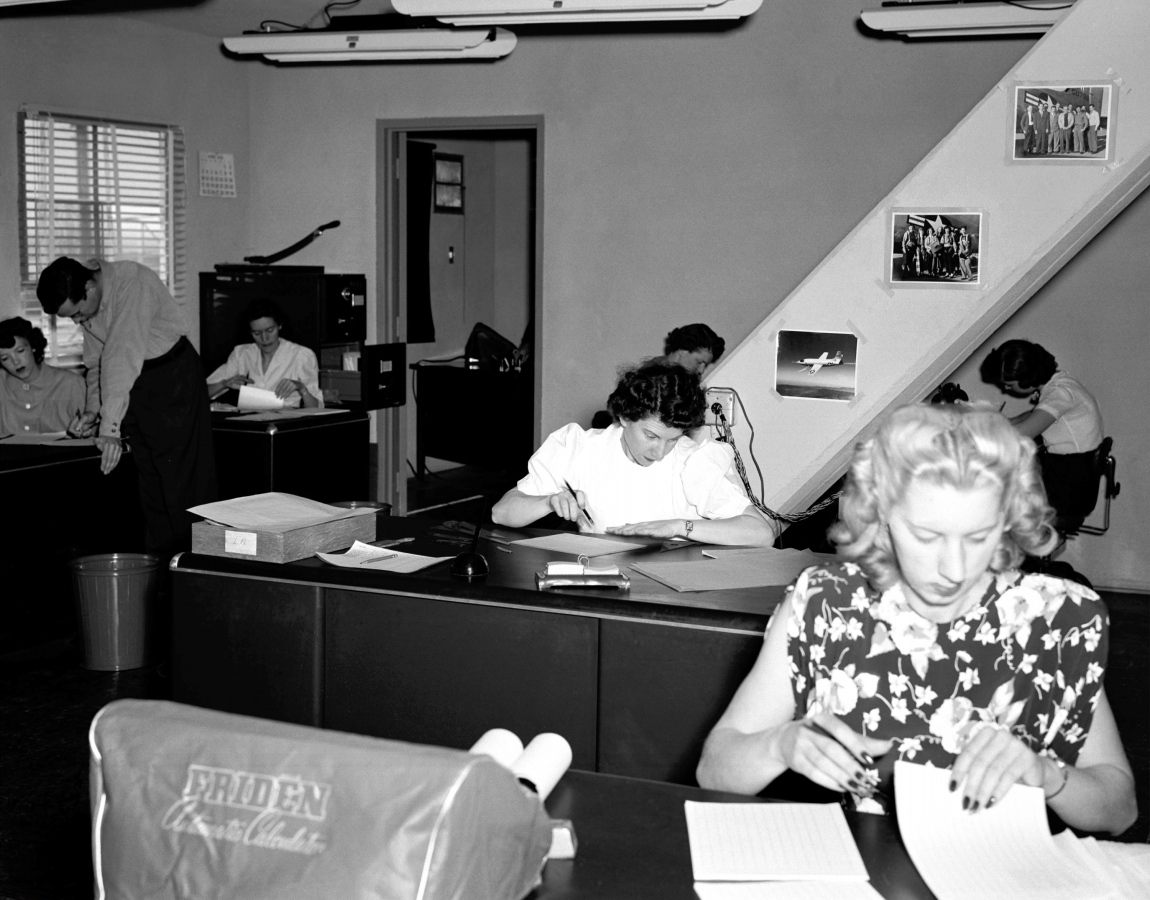
\includegraphics[height=15mm]{img/human-computers-1949.jpg}};
    \draw[ruling, line width=0.4pt] ([shift={(-1.2,1.2)}]photo.north west) rectangle
      ([shift={(1.2,-1.2)}]photo.south east);
    \draw[brand, line width=1pt, line join=miter] (80.5,0) rectangle (124.5,-15);
    \node[part, minimum width=14mm, minimum height=6mm] (grace) at (90.5,-5.5) {Grace};
    \node[part, draw=brand, minimum width=14mm, minimum height=6mm] (hopper) at (114.5,-5.5) {Hopper};
    \draw[flow both] (grace) to (hopper);
    \node[font=\footnotesize, text=muted, inner sep=0] at (102.5,-11.8) {96 GB HBM3};
    % the table: a header, three rows of 4.4 mm and the food row of 8.2 mm (the last row 3.8 mm taller)
    \renewcommand{\cxsheetextra}{3.8}
    \cxsheet{0}{-18}{20}{55}{2}{4}{4.4}{4.8}
    \node[shead] at (47.5,-20.4) {Human computer, 1949};
    \node[shead] at (102.5,-20.4) {One GH200, 2024};
    \foreach \y/\n/\lab/\a/\b in {%
        -25.0/2/{Rate}/{1,000 additions a day}/{$990 \times 10^{12}$ FLOP/s},
        -29.4/3/{Format}/{Decimal, by hand}/{16 bits per number},
        -33.8/4/{Power}/{About 100 W}/{660 W on Alps}} {
      \node[slab, font=\small\itshape, text=muted, anchor=west, visible on=<\n->] at (2,\y) {\lab};
      \node[scell, visible on=<\n->] at (47.5,\y) {\a};
      \node[scell, visible on=<\n->] at (102.5,\y) {\b};}
    % the food row: the wattage said as food, the only unit here that a room can feel
    \node[slab, font=\small\itshape, text=muted, anchor=west, visible on=<5->] at (2,-40.1) {Food};
    \node[scell, visible on=<5->] at (47.5,-40.1)
      {\textcolor{brand}{\bfseries 2,065 kcal a day}\\ {\footnotesize\itshape\color{muted}what one person eats}};
    \node[scell, visible on=<5->] at (102.5,-40.1)
      {\textcolor{brand}{\bfseries 13,600 kcal a day}\\ {\footnotesize\itshape\color{muted}what six or seven people eat}};
    \node[body, font=\small, anchor=north west, text width=130mm, visible on=<6->] at (0,-45.6)
      {The clerk's rate is what the shop \emph{delivered}. The chip's is what it \emph{could} do.};
    \cxsrc{Photograph: a computer room, NACA, 1949 (NASA Dryden, E49-54), public domain.}
  \end{tikzpicture}
\end{frame}

% ===== A GH200 is a CPU and a GPU on one module (FDD slide 13). The three FDD bullets are glosses.
\begin{frame}{A GH200 is a CPU and a GPU on one module}
  \begin{tikzpicture}[x=1mm, y=1mm]
    \path[use as bounding box] (0,1) rectangle (130,-54);
    \draw[brand, line width=1.2pt, line join=miter] (1,-4) rectangle (71,-44);
    \node[box, text width=20mm, visible on=<2->] (grace) at (15.4,-19) {\textbf{Grace}\\ an ARM CPU};
    \node[box strong, text width=25mm, visible on=<3->] (hopper) at (53.5,-19)
      {\textbf{Hopper}\\ the GPU that does\\ the arithmetic};
    \draw[flow both, visible on=<4->] (grace.east) to (grace.east -| hopper.west);
    \node[lbl, anchor=north, visible on=<4->] at (34,-32) {one fast internal link};
    \node[font=\normalsize, text=ink, inner sep=0, visible on=<5->] at (36,-39.5) {96 GB of HBM3 at 4 TB/s};
    \node[gloss, anchor=north west, visible on=<6->] at (76,-2)
      {The GPU computes. The CPU reads the data, runs Python, and keeps it fed};
    \node[gloss, anchor=north west, visible on=<7->] at (76,-18.5)
      {HBM3 is memory stacked on the GPU package: only 96 GB, but 4 TB/s};
    \node[gloss, anchor=north west, visible on=<8->] at (76,-35)
      {Between them 900 GB/s, about seven times what a plug-in card gets};
  \end{tikzpicture}
\end{frame}

% ===== Alps is an HPE Cray EX254n (FDD slide 14), with a picture of the platform and its blades
% ===== alps-platform-frame.tex: "Alps is an HPE Cray EX254n" (FDD slide 14), input by block5-computing-clusters.tex
% Carlos, 2026-11-10: "try to make a diagram that shows how the supercomputer platform looks and then the blade
% types inside it". Two frames: the platform as a zoom from a cabinet to a chassis to one blade, then the blade
% types of the platform drawn side by side.
% Facts, checked on 2026-11-10 against HPE's QuickSpecs (version 22, 21 September 2026, a00094635enw) and CSCS's
% hardware page (docs.cscs.ch/alps/hardware):
%   a cabinet holds 8 chassis; a chassis has 8 compute blade slots ("up to 64 compute blade slots across eight
%   compute chassis"); Alps's GH200 chassis use 7 of the 8 ("underpopulated so that we can increase the amount
%   of power delivered to each GPU"), so 56 blades, 112 nodes and 448 GH200 a cabinet, 24 cabinets;
%   EX254n: "Two 4-socket Nvidia GH200 Grace Hopper Superchip nodes", one node per board.
%   The blades of frame 2, from the same QuickSpecs and its 2021 version 4: EX235n, two nodes of 4 NVIDIA A100 and
%   1 AMD EPYC; EX235a, two nodes of 4 AMD MI250X and 1 AMD EPYC; EX255a, two nodes of 4 AMD MI300A; EX4252, four
%   nodes of 2 AMD EPYC. EX425, EX235a and EX235n are discontinued (version 22 change log); Alps still runs EX235a
%   blades, and CSCS names EX255A as well.
%   FDD's line "The trailing n marks the NVIDIA accelerated blades" is HPE's pattern, never its stated rule, so
%   the frame says only what the five names show.
%   Left out: the cabinet's model (CSCS writes EX3000, HPE defines EX4000), rectifier counts, the number of CDUs.

% ===== Frame 1. The platform, from a cabinet to one blade
\begin{frame}{Alps is an HPE Cray EX254n}
  \begin{tikzpicture}[x=1mm, y=1mm]
    \path[use as bounding box] (0,1) rectangle (130,-54);
    \node[body, font=\small, anchor=north west, text width=130mm] at (0,0)
      {The TOP500 entry reads: \emph{Alps, HPE Cray EX254n, NVIDIA Grace 72C 3.1GHz, NVIDIA GH200 Superchip,
       Slingshot-11, HPE Cray OS}};
    % the platform: one cabinet, its 8 chassis
    \begin{scope}[visible on=<2->]
      \node[font=\small\bfseries, text=ink, anchor=base, inner sep=0] at (37,-13.6) {HPE Cray EX, the platform};
      \draw[nib, line width=0.7pt, line join=miter] (0,-15.5) rectangle (22,-36.5);
      \foreach \k in {0,...,7} {
        \draw[nib, line width=0.45pt, line join=miter] (1.6,{-16.6-\k*2.375}) rectangle (20.4,{-18.4-\k*2.375});}
      \node[font=\footnotesize\itshape, text=muted, anchor=north, align=center, inner sep=0] at (11,-38.2)
        {one of 24 cabinets:\\ 8 chassis};
    \end{scope}
    % one chassis: 8 blade slots, 7 used at Alps
    \begin{scope}[visible on=<3->]
      \draw[brand, line width=1.1pt, line join=miter] (1.6,-21.35) rectangle (20.4,-23.15);
      \draw[zoom] (20.4,-21.35) to (30,-15.5) (20.4,-23.15) to (30,-36.5);
      \draw[nib, line width=0.7pt, line join=miter] (30,-15.5) rectangle (74,-36.5);
      \foreach \k in {0,...,6} {
        \draw[nib, line width=0.5pt, line join=miter, fill=paper] (32,{-16.6-\k*2.375}) rectangle (72,{-18.3-\k*2.375});}
      \draw[muted, line width=0.5pt, dash pattern=on 1.6pt off 1.2pt] (32,{-16.6-7*2.375}) rectangle (72,{-18.3-7*2.375});
      \node[font=\footnotesize\itshape, text=muted, anchor=north, align=center, inner sep=0] at (52,-38.2)
        {one chassis: 8 blade slots,\\ 7 used at Alps, for more power per GPU};
    \end{scope}
    % one EX254n blade: two nodes of four GH200
    \begin{scope}[visible on=<4->]
      \draw[brand, line width=1.1pt, line join=miter] (32,-18.975) rectangle (72,-20.675);
      \draw[zoom] (72,-18.975) to (82,-15.5) (72,-20.675) to (82,-36.5);
      \node[font=\small\bfseries, text=brand, anchor=base, inner sep=0] at (106,-13.6) {EX254n, the blade};
      \draw[nib, line width=0.7pt, line join=miter] (82,-15.5) rectangle (130,-36.5);
      \foreach \bx in {84,107} {
        \draw[ruledark, line width=0.5pt, line join=miter] (\bx,-17.4) rectangle ({\bx+21},-30.4);
        \foreach \i in {0,1} {\foreach \j in {0,1} {
          \fill[hatch] ({\bx+2.5+\i*9},{-19.2-\j*5.6}) rectangle ({\bx+9.5+\i*9},{-23.2-\j*5.6});
          \draw[brand, line width=0.55pt, line join=miter]
            ({\bx+2.5+\i*9},{-19.2-\j*5.6}) rectangle ({\bx+9.5+\i*9},{-23.2-\j*5.6});}}
        \node[font=\footnotesize\itshape, text=muted, anchor=north, inner sep=0] at ({\bx+10.5},-31.4) {node};}
      \node[font=\footnotesize\itshape, text=muted, anchor=north, align=center, inner sep=0] at (106,-38.2)
        {2 nodes $\times$ 4 GH200\\ $=$ 8 GH200 a blade};
    \end{scope}
    \node[body, font=\small, anchor=north west, text width=130mm, visible on=<5->] at (0,-47.8)
      {The platform: cabinets, liquid cooling, power and the network.};
  \end{tikzpicture}
\end{frame}

% ===== Frame 2. The blade types of the platform. A hatched square is a GPU, or a module that carries one
% (GH200 and MI300A put a CPU and a GPU on one package); a plain square is a CPU.
\newcommand{\cxblade}[6]{% overlay, y centre, name, maker, nodes (2 or 4), style: gh (4 GPU modules),
  % gc (4 GPUs and 1 CPU), cpu (2 CPUs)
  \begin{scope}[visible on=<#1>]
    \node[font=\small\bfseries, text=ink, anchor=base west, inner sep=0] at (0,{#2+0.6}) {#3};
    \node[font=\footnotesize\itshape, text=muted, anchor=north west, inner sep=0] at (0,{#2-0.6}) {#4};
    \pgfmathsetmacro{\cxbw}{100/#5}%
    \foreach \nd in {1,...,#5} {
      \pgfmathsetmacro{\cxbl}{30+(\nd-1)*\cxbw}%
      \draw[ruledark, line width=0.45pt, line join=miter] ({\cxbl+0.8},{#2+2.2}) rectangle ({\cxbl+\cxbw-0.8},{#2-2.2});
      \ifx#6g
        \foreach \q in {0,...,3} {
          \pgfmathsetmacro{\cxqx}{\cxbl+\cxbw/2-9.2+\q*4.8}%
          \fill[hatch] (\cxqx,{#2+1.6}) rectangle ({\cxqx+3.6},{#2-1.6});
          \draw[brand, line width=0.5pt, line join=miter] (\cxqx,{#2+1.6}) rectangle ({\cxqx+3.6},{#2-1.6});}
      \fi
      \ifx#6c
        \foreach \q in {0,...,3} {
          \pgfmathsetmacro{\cxqx}{\cxbl+\cxbw/2-11.6+\q*4.8}%
          \fill[hatch] (\cxqx,{#2+1.6}) rectangle ({\cxqx+3.6},{#2-1.6});
          \draw[brand, line width=0.5pt, line join=miter] (\cxqx,{#2+1.6}) rectangle ({\cxqx+3.6},{#2-1.6});}
        \pgfmathsetmacro{\cxqx}{\cxbl+\cxbw/2-11.6+4*4.8}%
        \draw[nib, line width=0.5pt, line join=miter, fill=paper] (\cxqx,{#2+1.6}) rectangle ({\cxqx+3.6},{#2-1.6});
      \fi
      \ifx#6u
        \foreach \q in {0,1} {
          \pgfmathsetmacro{\cxqx}{\cxbl+\cxbw/2-4.2+\q*4.8}%
          \draw[nib, line width=0.5pt, line join=miter, fill=paper] (\cxqx,{#2+1.6}) rectangle ({\cxqx+3.6},{#2-1.6});}
      \fi
    }
  \end{scope}}

\begin{frame}{One platform, several blade types}
  \begin{tikzpicture}[x=1mm, y=1mm]
    \path[use as bounding box] (0,1) rectangle (130,-54);
    % the key
    \fill[hatch] (86,-0.4) rectangle (89.6,-3.6);
    \draw[brand, line width=0.5pt, line join=miter] (86,-0.4) rectangle (89.6,-3.6);
    \node[font=\footnotesize, text=ink, anchor=west, inner sep=0] at (90.8,-2) {a GPU};
    \draw[nib, line width=0.5pt, line join=miter, fill=paper] (106,-0.4) rectangle (109.6,-3.6);
    \node[font=\footnotesize, text=ink, anchor=west, inner sep=0] at (110.8,-2) {a CPU};
    \node[font=\footnotesize\itshape, text=muted, anchor=west, inner sep=0] at (30,-2) {each box is one node of a blade};
    % the blades
    \cxblade{1-}{-7}{EX254n}{NVIDIA GH200}{2}{g}
    \draw[brand, line width=1.1pt, line join=miter] (30,-4.2) rectangle (130,-9.8);
    \cxblade{2-}{-14.2}{EX235n}{NVIDIA A100}{2}{c}
    \cxblade{2-}{-21.4}{EX235a}{AMD MI250X}{2}{c}
    \cxblade{2-}{-28.6}{EX255a}{AMD MI300A}{2}{g}
    \cxblade{3-}{-35.8}{EX4252}{AMD EPYC}{4}{u}
    \node[font=\small\itshape, text=muted, anchor=north west, inner sep=0, visible on=<4->] at (0,-41.6)
      {Every name here that ends in n carries NVIDIA GPUs.};
    \node[body, font=\small, anchor=north west, text width=130mm, visible on=<5->] at (0,-45.8)
      {The blade choice is what makes Alps a machine for AI\\ rather than a conventional CPU cluster.};
  \end{tikzpicture}
\end{frame}


% ===== The atelier against Alps (FDD slide 15): collection against collection
\begin{frame}{The atelier against Alps}
  \begin{tikzpicture}[x=1mm, y=1mm]
    \path[use as bounding box] (0,1) rectangle (130,-54);
    \cxsheet{0}{-4}{50}{40}{2}{2}{11}{6}
    \node[shead, anchor=west] at (2,-7) {A collection of computers};
    \node[shead] at (70,-7) {Rate};
    \node[shead] at (110,-7) {Power};
    \node[slab, anchor=west] at (2,-15.5) {Prony's atelier, 1795\\ twenty people};
    \node[scell] at (70,-15.5) {0.694 additions/s};
    \node[scell] at (110,-15.5) {about 2 kW};
    \node[slab, anchor=west, visible on=<2->] at (2,-26.5) {Alps, 2024\\ 10,752 modules};
    \node[scell, visible on=<2->] at (70,-26.5) {$10.64 \times 10^{18}$ FLOP/s};
    \node[scell, visible on=<2->] at (110,-26.5) {7.1 MW};
    \node[body, font=\normalsize\bfseries, text=brand, anchor=north west, text width=130mm, visible on=<3->]
      at (0,-38) {Fifteen billion billion times the rate,\\ on three and a half thousand times the power};
  \end{tikzpicture}
\end{frame}

% ===== CSCS and Alps, the machine behind Apertus (FDD slide 17). Carlos, 2026-11-10: "Don't say that at
% dense BF16 the whole partition is about 10.6 EFLOP/s. Simply say 10.6 EFLOP/s and give in decimal notation
% how many flops that is", and drop the TOP500 sentence. FDD's title said "the anchor", Apertus, which its
% dropped frame "The anchor: Apertus, trained on Alps" introduced; the last line here introduces it instead.
\begin{frame}{CSCS and Alps, the machine behind Apertus}
  \begin{tikzpicture}[x=1mm, y=1mm]
    \path[use as bounding box] (0,1) rectangle (130,-54);
    \node[box quiet, text width=36mm] (cscs) at (21,-10.5)
      {\textbf{CSCS}\\ the Swiss National\\ Supercomputing\\ Centre, Lugano};
    \node[box, text width=28mm, visible on=<2->] (alps) at (64,-10.5) {\textbf{Alps}\\ HPE Cray EX254n};
    \draw[flow, visible on=<2->] (cscs) to (alps);
    \node[box strong, text width=30mm, visible on=<3->] (count) at (110,-10.5)
      {2,688 nodes\\ $\times$ 4 GH200\\ $=$ 10,752 sockets};
    \draw[flow, visible on=<3->] (alps) to (count);
    \node[big, anchor=base west, visible on=<4->] at (0,-30.5) {10.6 EFLOP/s};
    \node[font=\LARGE, text=brand, inner sep=0, anchor=base west, visible on=<4->] at (41,-30.5)
      {$= 10.6 \times 10^{18}$ FLOP/s};
    \node[measure, anchor=base west, visible on=<4->] at (0,-36) {all 10,752 GH200 together};
    \node[body, anchor=north west, text width=130mm, visible on=<5->] at (0,-39.6)
      {Apertus, the open language model of EPFL, ETH Zurich and CSCS, was trained on Alps.};
    \cxsrc{Machine: \weblink{https://www.cscs.ch/computers/alps}{cscs.ch/computers/alps} and
      \weblink{https://www.top500.org/system/180259/}{top500.org/system/180259}.\quad Model: \arxiv{2509.14233}.}
  \end{tikzpicture}
\end{frame}

% ===== Nodes and sockets (FDD slide 30, moved here by Carlos: "it fits better there")
\begin{frame}{Nodes and sockets}
  \begin{tikzpicture}[x=1mm, y=1mm]
    \path[use as bounding box] (0,1) rectangle (130,-54);
    \draw[brand, line width=1.2pt, line join=miter] (2,-5) rectangle (62,-19);
    \node[font=\small\bfseries, text=brand, anchor=base west, inner sep=0] at (2,-3.4) {One node};
    \foreach \i in {0,1,2,3} {
      \node[part, minimum width=11mm, minimum height=9mm, visible on=<2->] at (12+\i*13.33,-12) {GH200};}
    \node[lbl, anchor=north, visible on=<2->] at (32,-21) {One operating system, one address space};
    \node[body, anchor=north west, text width=60mm, visible on=<3->] at (70,-5)
      {\textbf{Socket}\enspace one processor module\\[1.2mm] \textbf{Node}\enspace one independent computer};
    \node[box strong, text width=100mm, visible on=<4->] at (65,-30.5)
      {2,688 nodes $\times$ 4 modules $=$ 10,752 sockets};
    \node[body, font=\small, anchor=north west, visible on=<5->] at (0,-38.2)
      {Socket to socket, inside the node: \textbf{150 GB/s}};
    \node[body, font=\small, text=bad, anchor=north west, visible on=<6->] at (0,-43)
      {Between nodes: \textbf{25 GB/s} per GPU, six times less};
    \node[body, font=\small, anchor=north west, visible on=<7->] at (0,-48.6)
      {The node boundary is where the bandwidth falls off.};
  \end{tikzpicture}
\end{frame}

% ===== One second of a GH200, in three registers (FDD slide 18)
\begin{frame}{One second of a GH200, in three registers}
  \begin{tikzpicture}[x=1mm, y=1mm]
    \path[use as bounding box] (0,1) rectangle (130,-54);
    \cxsheet{0}{-3}{92}{38}{1}{3}{12}{6}
    \node[shead, anchor=west] at (2,-6) {The same one second of arithmetic};
    \node[shead] at (111,-6) {Time};
    \node[slab, anchor=west] at (2,-15)
      {The mean age of all 8.2 billion people alive,\\ one addition each};
    \node[scell, font=\normalsize\bfseries, text=brand] at (111,-15) {8.3 microseconds};
    \node[slab, anchor=west, visible on=<2->] at (2,-27)
      {130,000 photographs classified by ResNet-50,\\ each 224 by 224 pixels, or 0.05 megapixels};
    \node[scell, font=\normalsize\bfseries, text=brand, visible on=<2->] at (111,-27) {one second};
    \node[slab, anchor=west, visible on=<3->] at (2,-39) {Prony's atelier doing that same\\ one second of work};
    \node[scell, font=\normalsize\bfseries, text=bad, visible on=<3->] at (111,-39) {45 to 136\\ million years};
    \cxsrc{ResNet-50: He and others, \arxiv{1512.03385}: 3.8 billion multiply-adds, so
      $7.6 \times 10^{9}$ FLOP per image. A peak count.}
  \end{tikzpicture}
\end{frame}

% ============================================================ section 2
% FDD's section 3 is cut but for these two frames (Carlos: "keep the slide capacity and bandwidth are
% different numbers, because that one I like. Then 246 operations per byte").
\section{What the headline rate hides}

% ===== Capacity and bandwidth are different numbers (FDD slide 25)
\begin{frame}{Capacity and bandwidth are different numbers}
  \begin{tikzpicture}[x=1mm, y=1mm]
    \path[use as bounding box] (0,1) rectangle (130,-54);
    \node[box, text width=54mm] at (32,-9) {{\Large\bfseries 96 GB}\\ how much fits};
    \node[box strong, text width=52mm, visible on=<2->] at (98,-9) {{\Large\bfseries 4 TB/s}\\ how fast you can move it};
    \node[body, font=\small, anchor=north west, text width=56mm, visible on=<3->] at (4,-22)
      {Decides whether the weights and the optimiser state fit on one device at all};
    \node[body, font=\small, anchor=north west, text width=56mm, visible on=<4->] at (70,-22)
      {Decides how quickly the arithmetic units can be fed once the data is there};
    \draw[rule, visible on=<5->] (0,-35) to (130,-35);
    \node[body, font=\small, anchor=north west, text width=130mm, visible on=<5->] at (0,-38)
      {96 GB is less than an ordinary server holds. That is the trade: HBM is stacked on the package and wired
       short and wide, which is what buys the speed.};
  \end{tikzpicture}
\end{frame}

% ===== Two hundred and forty six operations per byte (FDD slide 26): the arithmetic intensity
\begin{frame}{Two hundred and forty six operations per byte}
  \begin{tikzpicture}[x=1mm, y=1mm]
    \path[use as bounding box] (0,1) rectangle (130,-54);
    \node[box quiet, text width=22mm] (hbm) at (15.4,-8) {\textbf{HBM3}\\ 4 TB/s};
    \draw[draw=nib, line width=2.2pt, line join=miter, -{Triangle[length=3.4mm, width=2.8mm]},
      visible on=<2->] (hbm.east) to (83,-8);
    \node[lbl, anchor=north, visible on=<2->] at (56,-11) {the only way in};
    \node[box strong, text width=38mm, visible on=<3->] (units) at (106,-8)
      {\textbf{The arithmetic units}\\ $990 \times 10^{12}$ FLOP/s of appetite};
    \node[font=\normalsize, text=ink, inner sep=0, visible on=<4->] at (65,-25)
      {$\dfrac{990 \times 10^{12}\ \text{FLOP/s}}{4.023 \times 10^{12}\ \text{bytes/s}}
        \;=\; 246\ \text{FLOP per byte}$};
    \node[lbl, anchor=north, visible on=<5->] at (65,-31.5)
      {A rate over a rate: the seconds cancel, and what is left is operations per byte};
    \node[body, font=\small, anchor=north west, text width=130mm, visible on=<6->] at (0,-37.5)
      {So unless the computation reuses each byte about that many times, the units wait. A large matrix
       multiply does reuse. Many other operations do not.};
    \node[body, font=\small, anchor=north west, text width=130mm, visible on=<7->] at (0,-47.5)
      {This is one of the reasons a real run reaches 21 to 46 percent of peak.};
  \end{tikzpicture}
\end{frame}

% ============================================================ section 3
\section{The machine, and what it draws}

% ===== A watt is a rate, a kilowatt hour is an amount (FDD slide 28, first half: the tap and the glass).
% Carlos, 2026-11-10: "divide this into two slides. In one slide, have the glass of water. The other is about
% watching the slash", with the formulas rate times time, FLOP/s times seconds, watts times hours.
\begin{frame}{A watt is a rate, a kilowatt hour is an amount}
  \begin{tikzpicture}[x=1mm, y=1mm]
    \path[use as bounding box] (0,1) rectangle (130,-54);
    % the tap
    \draw[nib, line width=1.6pt, line join=miter] (24,-5) to (56,-5) to (56,-11);
    \draw[nib, line width=1.6pt] (40,-5) to (40,-1.2);
    \draw[nib, line width=1.6pt] (36.5,-1.2) to (43.5,-1.2);
    \node[big, anchor=west] at (72,-5) {660 W};
    \node[body, anchor=west] at (72,-12) {How fast energy arrives};
    \foreach \y in {-15,-19.5,-24} {\fill[brand, visible on=<2->] (56,\y) circle (1.1);}
    % the glass
    \fill[hatch, visible on=<3->] (47.6,-37) to (49,-48) to (63,-48) to (64.4,-37) to cycle;
    \draw[brand, line width=0.5pt, visible on=<3->] (47.6,-37) to (64.4,-37);
    \draw[nib, line width=1.6pt, line join=miter, visible on=<3->] (46,-27) to (49,-48) to (63,-48) to (66,-27);
    \node[big, anchor=west, visible on=<3->] at (72,-36) {0.66 kWh};
    \node[measure, anchor=west, visible on=<3->] at (100,-36.4) {after one hour};
    \node[body, anchor=west, visible on=<3->] at (72,-43) {How much arrived};
  \end{tikzpicture}
\end{frame}

% ===== Watch the slash (FDD slide 28, second half, and its closing bullet as three formulas)
\begin{frame}{Watch the slash}
  \begin{tikzpicture}[x=1mm, y=1mm]
    \path[use as bounding box] (0,1) rectangle (130,-54);
    \node[big, text=ink, anchor=base west] at (0,-6) {km\textcolor{brand}{/}h};
    \node[body, anchor=base west] at (30,-6) {The slash divides, so it is a speed.};
    \node[big, text=ink, anchor=base west, visible on=<2->] at (0,-17) {kWh};
    \node[body, anchor=base west, visible on=<2->] at (30,-17) {No slash. The hour \textbf{multiplies}, so it is an amount.};
    \node[body, text=bad, anchor=base west, visible on=<3->] at (30,-25)
      {Longer gives you \emph{more}, so the hour cannot be dividing.};
    \draw[rule, visible on=<4->] (0,-30.5) to (130,-30.5);
    % rate times time is an amount, twice over
    \foreach \y/\n/\a/\b/\c/\ink in {%
        -37/4/{rate}/{time}/{amount}/brand,
        -44/5/{FLOP/s}/{seconds}/{FLOP}/ink,
        -51/6/{watts}/{hours}/{watt hours}/ink} {
      \node[font=\large, text=\ink, anchor=base east, inner sep=0, visible on=<\n->] at (46,\y) {\a};
      \node[font=\large, text=muted, anchor=base, inner sep=0, visible on=<\n->] at (51,\y) {$\times$};
      \node[font=\large, text=\ink, anchor=base west, inner sep=0, visible on=<\n->] at (56,\y) {\b};
      \node[font=\large, text=muted, anchor=base, inner sep=0, visible on=<\n->] at (80,\y) {$=$};
      \node[font=\large, text=\ink, anchor=base west, inner sep=0, visible on=<\n->] at (85,\y) {\c};}
  \end{tikzpicture}
\end{frame}

% ===== A wattage becomes a bill in two multiplications (FDD slide 29)
\begin{frame}{A wattage becomes a bill in two multiplications}
  \begin{tikzpicture}[x=1mm, y=1mm]
    \path[use as bounding box] (0,1) rectangle (130,-54);
    % the configurable band: 450 W at x = 12, 1,000 W at x = 118
    \node[font=\small\bfseries, text=ink, anchor=north west, inner sep=0] at (0,0) {One module is just a band};
    \draw[bar plain] (12,-6) rectangle (118,-10.5);
    \node[font=\small, text=muted, anchor=east, inner sep=0] at (11,-8.25) {450 W};
    \node[font=\small, text=muted, anchor=west, inner sep=0] at (119,-8.25) {1,000 W};
    \fill[hatch, visible on=<2->] (12,-6) rectangle (52.47,-10.5);
    \draw[brand, line width=0.9pt, visible on=<2->] (52.47,-6) to (52.47,-13);
    \node[font=\small\bfseries, text=brand, anchor=north west, inner sep=0, visible on=<2->] at (53.5,-11.6)
      {Alps caps \emph{each module} at about 660 W};
    \node[lbl, anchor=north west, visible on=<3->] at (12,-16.4)
      {The operator chooses: near 1,000 W is faster, lower saves energy and cooling};
    % the two multiplications
    \node[box, text width=26mm, visible on=<4->] (w) at (18,-27.6) {660 W\\ for one hour};
    \node[box, text width=26mm, visible on=<5->] (e) at (63,-27.6) {$=$ 0.66 kWh\\ of energy};
    \node[box strong, text width=28mm, visible on=<6->] (p) at (109,-27.6) {$=$ 5.3 Rappen\\ of electricity};
    \draw[flow, visible on=<5->] (w) to (e);
    \draw[flow, visible on=<6->] (e) to (p);
    \node[lbl, anchor=south, visible on=<5->] at (40.5,-26.7) {$\times$ time};
    \node[lbl, anchor=south, visible on=<6->] at (85.5,-26.7) {$\times$ price};
    \node[body, font=\small, anchor=north west, text width=130mm, visible on=<7->] at (0,-35.4)
      {That is \hl{one module}. All 10,752 is 7.1 megawatts, about 570 francs an hour.};
    \node[body, font=\small, anchor=north west, text width=130mm, visible on=<8->] at (0,-40)
      {The whole Apertus run is 3.96 GWh, about 0.3 million francs.};
    \node[src, anchor=north west, text width=130mm, visible on=<6->] at (0,-45)
      {450 to 1,000 W: GH200 datasheet. 660 W: the Alps cap,
      \weblink{https://docs.cscs.ch/running/slurm/}{docs.cscs.ch/running/slurm}. 8 Rappen per kWh assumed
      (ElCom 2026, large consumers 6.75 to 9; households pay 27.7). Check: 10,752 $\times$ 660 W is 7,096 kW,
      against the 7,124 kW the TOP500 measured.};
  \end{tikzpicture}
\end{frame}

% ===== Four links, and each step down costs you (FDD slide 31, drawn). Carlos, 2026-11-10: "make a diagram
% showing the supercomputer divided into nodes, the nodes divided into sockets, the sockets divided into
% Grace Hoppers, and then inside the GPU ... point at each link in the diagram that is connecting two
% components, and then report there the speed."
% Four panels, each a zoom into the part outlined in violet in the panel before. Clicks 1 to 4 build the
% machine from the outside in; clicks 5 to 8 give the speeds from the fastest link out, as FDD listed them.
\begin{frame}{Four links, and each step down costs you}
  \begin{tikzpicture}[x=1mm, y=1mm]
    \path[use as bounding box] (0,1) rectangle (130,-54);
    % panel 1: Alps, its nodes
    \node[font=\small\bfseries, text=ink, anchor=base, inner sep=0] at (13,-4.4) {Alps};
    \draw[nib, line width=0.6pt, line join=miter] (0,-6.5) rectangle (26,-28.5);
    \node[part, minimum width=9mm, minimum height=10mm] at (6.5,-17.5) {node};
    \node[part, minimum width=9mm, minimum height=10mm] at (20.5,-17.5) {node};
    \draw[link] (11,-17.5) to (16,-17.5);
    % panel 2: one node, its sockets
    \begin{scope}[visible on=<2->]
      \draw[brand, line width=1.1pt, line join=miter] (16,-12.5) rectangle (25,-22.5);
      \draw[zoom] (25,-12.5) to (30.333,-6.5) (25,-22.5) to (30.333,-28.5);
      \node[font=\small\bfseries, text=ink, anchor=base, inner sep=0] at (43.833,-4.4) {One node};
      \draw[nib, line width=0.6pt, line join=miter] (30.333,-6.5) rectangle (57.333,-28.5);
      \node[part, minimum width=10.5mm, minimum height=10mm] at (36.583,-17.5) {socket};
      \node[part, minimum width=10.5mm, minimum height=10mm] at (51.083,-17.5) {socket};
      \draw[link] (41.833,-17.5) to (45.833,-17.5);
    \end{scope}
    % panel 3: one socket, a GH200: Grace and Hopper
    \begin{scope}[visible on=<3->]
      \draw[brand, line width=1.1pt, line join=miter] (45.833,-12.5) rectangle (56.333,-22.5);
      \draw[zoom] (56.333,-12.5) to (61.667,-6.5) (56.333,-22.5) to (61.667,-28.5);
      \node[font=\small\bfseries, text=ink, anchor=base, inner sep=0] at (76.667,-4.4) {One socket};
      \draw[nib, line width=0.6pt, line join=miter] (61.667,-6.5) rectangle (91.667,-28.5);
      \node[part, minimum width=11mm, minimum height=10mm] at (68.167,-17.5) {Grace};
      \node[part, minimum width=12.5mm, minimum height=10mm] at (84.417,-17.5) {Hopper};
      \draw[link] (73.667,-17.5) to (78.167,-17.5);
    \end{scope}
    % panel 4: inside the GPU: its memory and its arithmetic units
    \begin{scope}[visible on=<4->]
      \draw[brand, line width=1.1pt, line join=miter] (78.167,-12.5) rectangle (90.667,-22.5);
      \draw[zoom] (90.667,-12.5) to (96,-6.5) (90.667,-22.5) to (96,-28.5);
      \node[font=\small\bfseries, text=ink, anchor=base, inner sep=0] at (113,-4.4) {Inside the GPU};
      \draw[nib, line width=0.6pt, line join=miter] (96,-6.5) rectangle (130,-28.5);
      \node[part, minimum width=11mm, minimum height=10mm] at (102.75,-17.5) {HBM3};
      \node[part, minimum width=16mm, minimum height=10mm] at (120.75,-17.5) {arithmetic\\ units};
      \draw[link] (108.25,-17.5) to (112.75,-17.5);
    \end{scope}
    % the speeds, each on a leader to its link, from the fastest out
    \foreach \x/\n/\v/\w in {%
        110.5/5/{4,023 GB/s}/{the GPU to its HBM3},
        75.917/6/{900 GB/s}/{Grace to Hopper},
        43.833/7/{150 GB/s}/{socket to socket},
        13.5/8/{25 GB/s per GPU}/{between nodes}} {
      \draw[leader, visible on=<\n->] (\x,-31.6) to (\x,-17.5);
      \fill[brand, visible on=<\n->] (\x,-17.5) circle (0.75);
      \node[font=\normalsize\bfseries, text=brand, anchor=north, inner sep=0, visible on=<\n->] at (\x,-32.4) {\v};
      \node[font=\footnotesize\itshape, text=muted, anchor=north, align=center, inner sep=0,
        visible on=<\n->] at (\x,-37.4) {\w};}
    \node[font=\small\bfseries, text=bad, anchor=north west, inner sep=0, visible on=<9->] at (0,-45)
      {Each step down costs about a factor of five. End to end, 161 times.};
    \node[body, font=\small, anchor=north west, inner sep=0, visible on=<10->] at (0,-50)
      {So you keep the data at the fast end and cross the slow links as rarely as you can.};
  \end{tikzpicture}
\end{frame}

% ============================================================ section 4
\section{From a model to GPU hours}

% ===== Two numbers price a training run (FDD slide 33). Carlos: present the 6ND rule "but replace training
% tokens by training numbers". The formula is set whole, its terms revealed in place, so nothing moves.
\begin{frame}{Two numbers price a training run}
  \begin{tikzpicture}[x=1mm, y=1mm]
    \path[use as bounding box] (0,1) rectangle (130,-54);
    \node[box, text width=38mm] (n) at (21.4,-5) {$N$ parameters};
    \node[box, text width=38mm] (d) at (21.4,-19) {$D$ training numbers};
    \node[box strong, text width=50mm, visible on=<2->] (c) at (98,-12) {$C$, the total training cost,\\ in FLOPs};
    \draw[flow, visible on=<2->] (n.east) -| (58,-10) to (c.west |- 0,-10);
    \draw[flow, visible on=<2->] (d.east) -| (58,-14) to (c.west |- 0,-14);
    \node[font=\Large, text=ink, inner sep=0, anchor=north, visible on=<3->] at (65,-30)
      {$C \;=\; \visible<5->{\underbrace{6}_{\substack{\text{\footnotesize per parameter,}\\
        \text{\footnotesize per training number}}} \times{}}
        \underbrace{N}_{\text{\footnotesize parameters}}
        \visible<4->{{}\times \underbrace{D}_{\substack{\text{\footnotesize training}\\
        \text{\footnotesize numbers}}}}$};
    \cxsrc[6-]{\weblink{https://arxiv.org/abs/2001.08361}{Kaplan and others, 2020}, section 2.1. Here the 6 is a
      rule of thumb.}
  \end{tikzpicture}
\end{frame}

% ===== A million by a million is two minutes (FDD slide 34): the miniature
\begin{frame}{A million by a million is two minutes}
  \begin{tikzpicture}[x=1mm, y=1mm]
    \path[use as bounding box] (0,1) rectangle (130,-54);
    \node[box, text width=32mm] (n) at (18.4,-7) {$N = 10^{6}$\\ parameters};
    \node[box, text width=32mm] (d) at (18.4,-23) {$D = 10^{6}$\\ training numbers};
    \node[box strong, text width=34mm, visible on=<2->] (c) at (64,-15) {$C = 6ND$\\ $= 6.00 \times 10^{12}$ FLOP};
    \draw[flow, visible on=<2->] (n.east) -| (40.3,-13) to (c.west |- 0,-13);
    \draw[flow, visible on=<2->] (d.east) -| (40.3,-17) to (c.west |- 0,-17);
    \node[box quiet, text width=34mm, visible on=<3->] (lap) at (110.2,-15) {A laptop at roughly\\ $50 \times 10^{9}$ FLOP/s};
    \draw[flow, visible on=<3->] (c) to (lap);
    \node[big, visible on=<4->] (sec) at (64,-40) {120 seconds};
    \draw[flow, visible on=<4->] (lap.south) |- (sec.east);
  \end{tikzpicture}
\end{frame}

% ===== The same formula on Apertus-70B (FDD slide 36). Carlos: "drop the anchor ... and then simply show the
% formula on Apertus-70B". The anchor frame's model source is here; its run source is on the next frame.
\begin{frame}{The same formula on Apertus-70B}
  \begin{tikzpicture}[x=1mm, y=1mm]
    \path[use as bounding box] (0,1) rectangle (130,-54);
    \node[box, text width=32mm] (n) at (18.4,-7) {$N = 70 \times 10^{9}$\\ parameters};
    \node[box, text width=32mm] (d) at (18.4,-23) {$D = 15 \times 10^{12}$\\ training numbers};
    \node[box strong, text width=34mm, visible on=<2->] (c) at (64,-15) {$C = 6ND$\\ $= 6.30 \times 10^{24}$ FLOP};
    \draw[flow, visible on=<2->] (n.east) -| (40.3,-13) to (c.west |- 0,-13);
    \draw[flow, visible on=<2->] (d.east) -| (40.3,-17) to (c.west |- 0,-17);
    \node[box quiet, text width=34mm, visible on=<3->] (mini) at (110.2,-15) {$1.05 \times 10^{12}$ times\\ the miniature};
    \draw[flow, draw=muted, visible on=<3->] (c) to (mini);
    \draw[bad, line width=0.9pt, visible on=<4->] (c.south) to (64,-31.5);
    \node[font=\normalsize, text=bad, align=center, anchor=north, inner sep=0, visible on=<4->] at (64,-32.5)
      {Apertus's own per operation count is $6.74 \times 10^{24}$,\\ seven percent higher};
    \cxsrc{Model: \arxiv{2509.14233}.}
  \end{tikzpicture}
\end{frame}

% ===== From one GPU hour to the whole run (FDD slide 37). The 6 million GPU hours come from the run paper,
% which FDD cited on its dropped anchor frame; the first line says so here.
\begin{frame}{From one GPU hour to the whole run}
  \begin{tikzpicture}[x=1mm, y=1mm]
    \path[use as bounding box] (0,1) rectangle (130,-54);
    \node[body, anchor=north west, text width=130mm] at (0,0)
      {The run: training Apertus-70B on 15 trillion training numbers took over 6 million GPU hours, on up to
       4,096 GPUs.};
    \node[box, text width=54mm, visible on=<2->] at (32,-17.2) {4,096 GPUs flat out\\ for \textbf{61 days}};
    \node[box, text width=54mm, visible on=<3->] at (98,-17.2) {It spanned about 91 days,\\ so \textbf{2,747} on average};
    \node[lbl, anchor=north, align=center, text width=124mm, visible on=<4->] at (65,-24.6)
      {The gap is ramp up, restarts and smaller phases:\\ a campaign rarely runs at full width without a break};
    \node[box strong, text width=110mm, inner ysep=2.2mm, visible on=<5->] at (65,-42)
      {6 million GPU hours $\times$ 660 W $=$ \textbf{3.96 GWh}\\ $\times$ 8 Rappen $=$ \textbf{0.32 million francs}};
    \cxsrc{Run: \arxiv{2604.12973}.}
  \end{tikzpicture}
\end{frame}

% ============================================================ section 5
\section{Dollars and energy}

% ===== Six million hours, priced at cloud rates (FDD slide 45). Dollars: x = 22 + 2.2 m, m in millions.
\begin{frame}{Six million hours, priced at cloud rates}
  \begin{tikzpicture}[x=1mm, y=1mm]
    \path[use as bounding box] (0,1) rectangle (130,-54);
    \draw[draw=muted, line width=0.6pt] (22,-41) to (112,-41);
    \foreach \m/\lab in {0/{\$0}, 20/{\$20M}, 40/{\$40M}} {
      \draw[draw=muted, line width=0.6pt] ({22+\m*2.2},-41) to ({22+\m*2.2},-42.6);
      \node[font=\footnotesize, text=muted, anchor=north, inner sep=0] at ({22+\m*2.2},-43.6) {\lab};}
    \node[font=\small, text=ink, align=right, anchor=east, inner sep=0, visible on=<2->] at (20,-14)
      {The 70B run,\\ 6 million hours};
    \fill[hatch, visible on=<2->] (41.8,-11) rectangle (74.8,-17);
    \draw[bar plain, fill=none, visible on=<2->] (41.8,-11) rectangle (74.8,-17);
    \node[font=\footnotesize, text=muted, anchor=south, inner sep=0, visible on=<2->] at (41.8,-9.6) {\$9.0M};
    \node[font=\footnotesize, text=muted, anchor=south, inner sep=0, visible on=<2->] at (74.8,-9.6) {\$24.0M};
    \draw[flow, draw=muted, visible on=<3->] (35,-22) to (41.2,-17.8);
    \node[font=\small, text=ink, anchor=north east, inner sep=0, visible on=<3->] at (35,-22.6) {6M h $\times$ \$1.50};
    \draw[flow, draw=muted, visible on=<4->] (81.6,-22) to (75.4,-17.8);
    \node[font=\small, text=ink, anchor=north west, inner sep=0, visible on=<4->] at (81.6,-22.6) {6M h $\times$ \$4.00};
    \fill[ink, visible on=<5->] (55,-14) circle (1.3);
    \draw[flow, draw=muted, visible on=<5->] (55,-30) to (55,-15.6);
    \node[font=\small\bfseries, text=brand, anchor=north, inner sep=0, visible on=<5->] at (55,-30.6)
      {6M h $\times$ \$2.50 $=$ \$15.0M};
    \cxsrc[6-]{The \$1.50 to \$4.00 band is an H100 rental survey, November 2025.}
  \end{tikzpicture}
\end{frame}

% ===== The same hours, in gigawatt hours (FDD slide 46). Energy: x = 16 + 10 g, g in GWh.
\begin{frame}{The same hours, in gigawatt hours}
  \begin{tikzpicture}[x=1mm, y=1mm]
    \path[use as bounding box] (0,1) rectangle (130,-54);
    \node[box, text width=44mm] at (25,-7) {8.85 million GPU hours\\ 90 days $\times$ 4,096 GPUs};
    \node[font=\large, text=muted, inner sep=0, visible on=<2->] at (53.5,-7) {$\times$};
    \node[box, text width=32mm, visible on=<2->] at (76,-7) {560 W\\ per module};
    \node[font=\large, text=muted, inner sep=0, visible on=<3->] at (98.5,-7) {$=$};
    \node[box strong, text width=20mm, visible on=<3->] at (116,-7) {\textbf{4.95 GWh}};
    % the range over four sourced module figures
    \begin{scope}[visible on=<4->]
      \draw[draw=muted, line width=0.6pt] (16,-30) to (116,-30);
      \foreach \g in {0,2,4,6,8,10} {
        \draw[draw=muted, line width=0.6pt] ({16+\g*10},-30) to ({16+\g*10},-31.6);
        \node[font=\footnotesize, text=muted, anchor=north, inner sep=0] at ({16+\g*10},-32.6) {\g};}
      \node[font=\footnotesize, text=muted, anchor=west, inner sep=0] at (118,-30) {GWh};
      \fill[hatch] (50,-22) rectangle (102,-27);
      \draw[bar plain, fill=none] (50,-22) rectangle (102,-27);
      \node[font=\footnotesize, text=muted, anchor=east, inner sep=0] at (48.6,-24.5) {3.4};
      \node[font=\footnotesize, text=muted, anchor=west, inner sep=0] at (103.4,-24.5) {8.6};
      \fill[ink] (65.5,-24.5) circle (1.3);
      \node[font=\small, text=ink, anchor=south, inner sep=0] at (65.5,-20.6) {4.95};
    \end{scope}
    \node[body, anchor=north west, text width=130mm, visible on=<5->] at (0,-37.6)
      {About 1,100 Swiss households for a year, at 4,500 kWh each.};
    \node[src, anchor=north west, text width=130mm, visible on=<6->] at (0,-43.4)
      {Range 750 to 1,900 households, over four sourced module figures: \textbf{560 W}, tech report, \arxiv{2509.14233};
       \textbf{660 W}, CSCS cap, \weblink{https://docs.cscs.ch/running/slurm/}{docs.cscs.ch/running/slurm};
       \textbf{855 W}, from the TOP500 run; datasheet band 450 to 1,000 W. Household 4,500 kWh a year is ElCom's
       H4 profile. CSCS publish a PUE below 1.2, cooling from Lake Lugano
       (\weblink{https://www.cscs.ch/computers/alps}{cscs.ch}).};
  \end{tikzpicture}
\end{frame}

\end{document}
